\chapter{Introduction}\label{ch:intro}
\begin{center}
 \rule[-4pt]{0.5pt}{4pt}\hrulefill\rule[-4pt]{0.5pt}{4pt}\\
 \begin{minipage}[c]{.33\linewidth}
  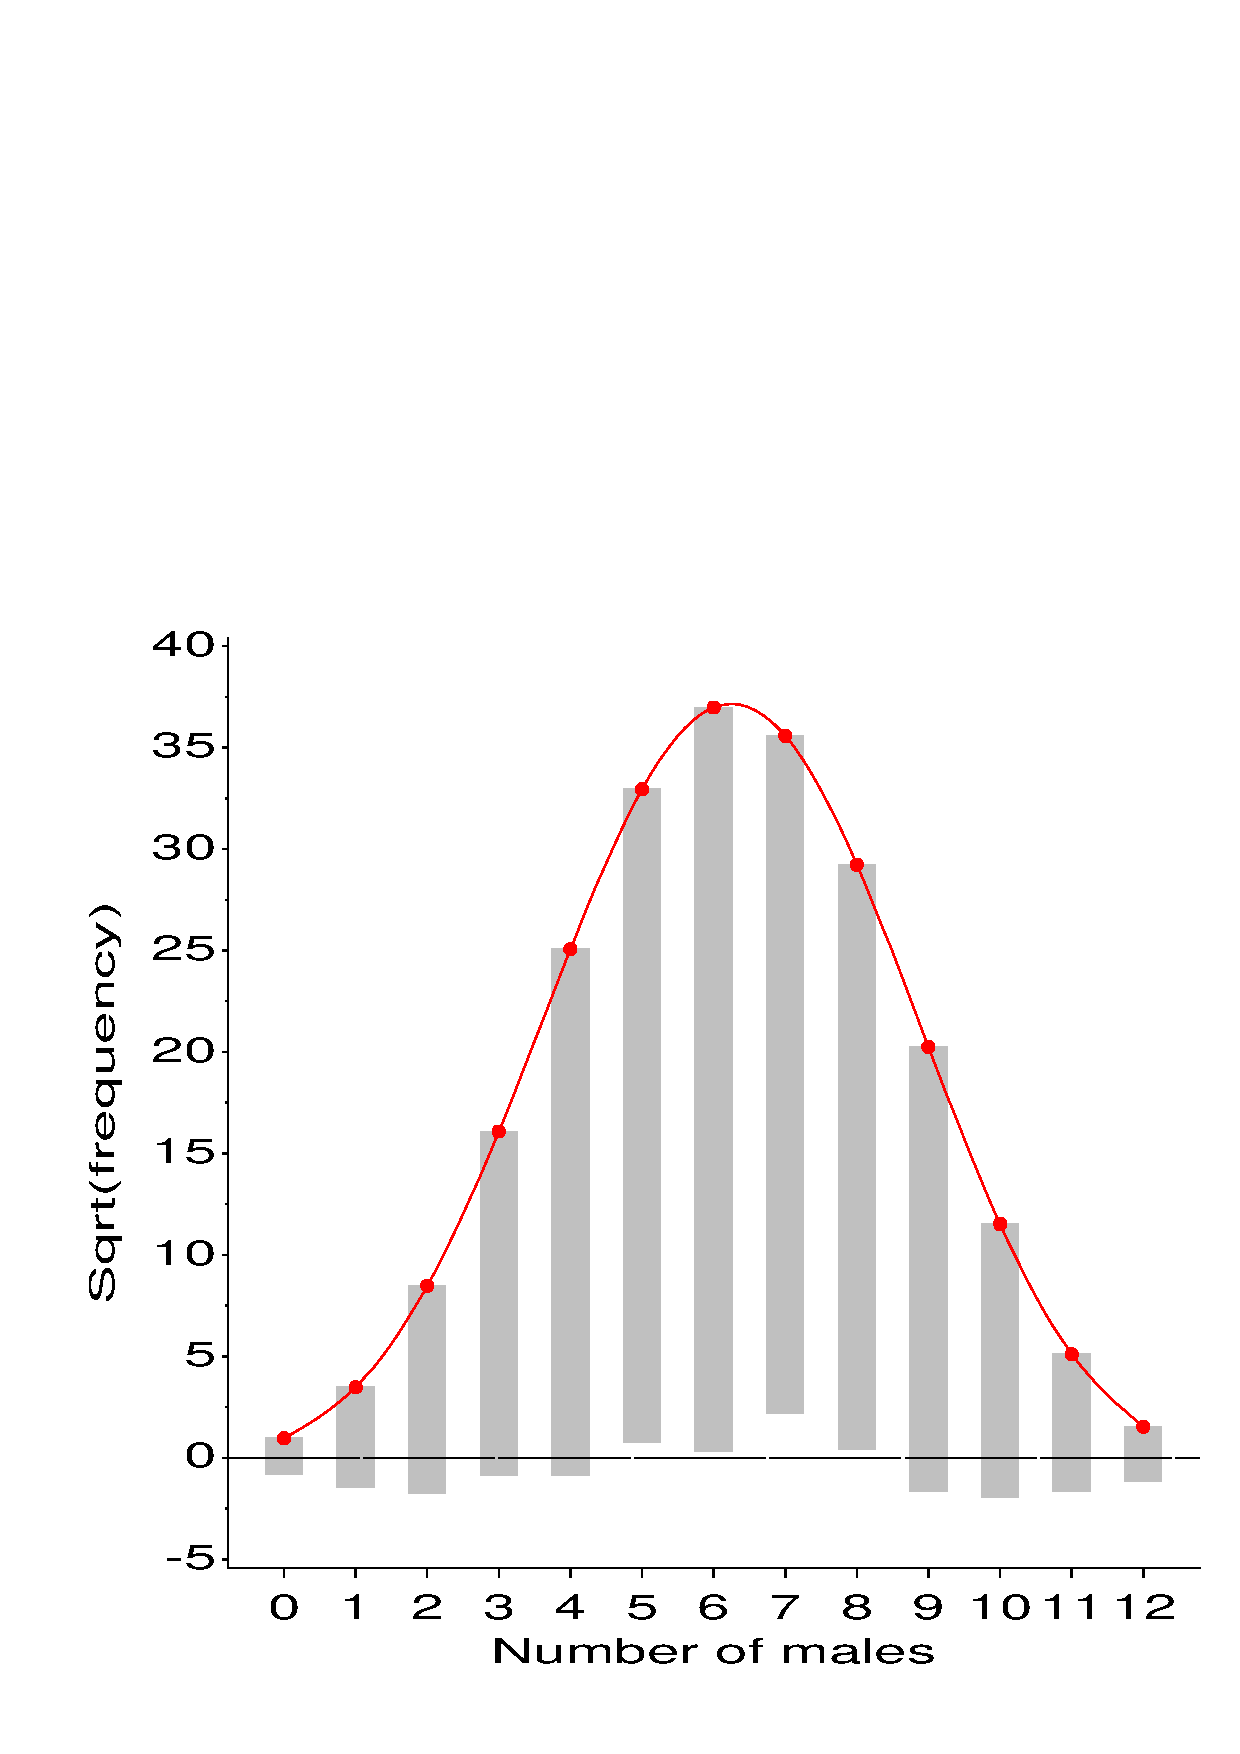
\includegraphics[width=1\linewidth]{saxony}\graphicsfile{ch2/fig/saxony.eps}{}
 \end{minipage}%
 \hfill
 \begin{minipage}[c]{.33\linewidth}
  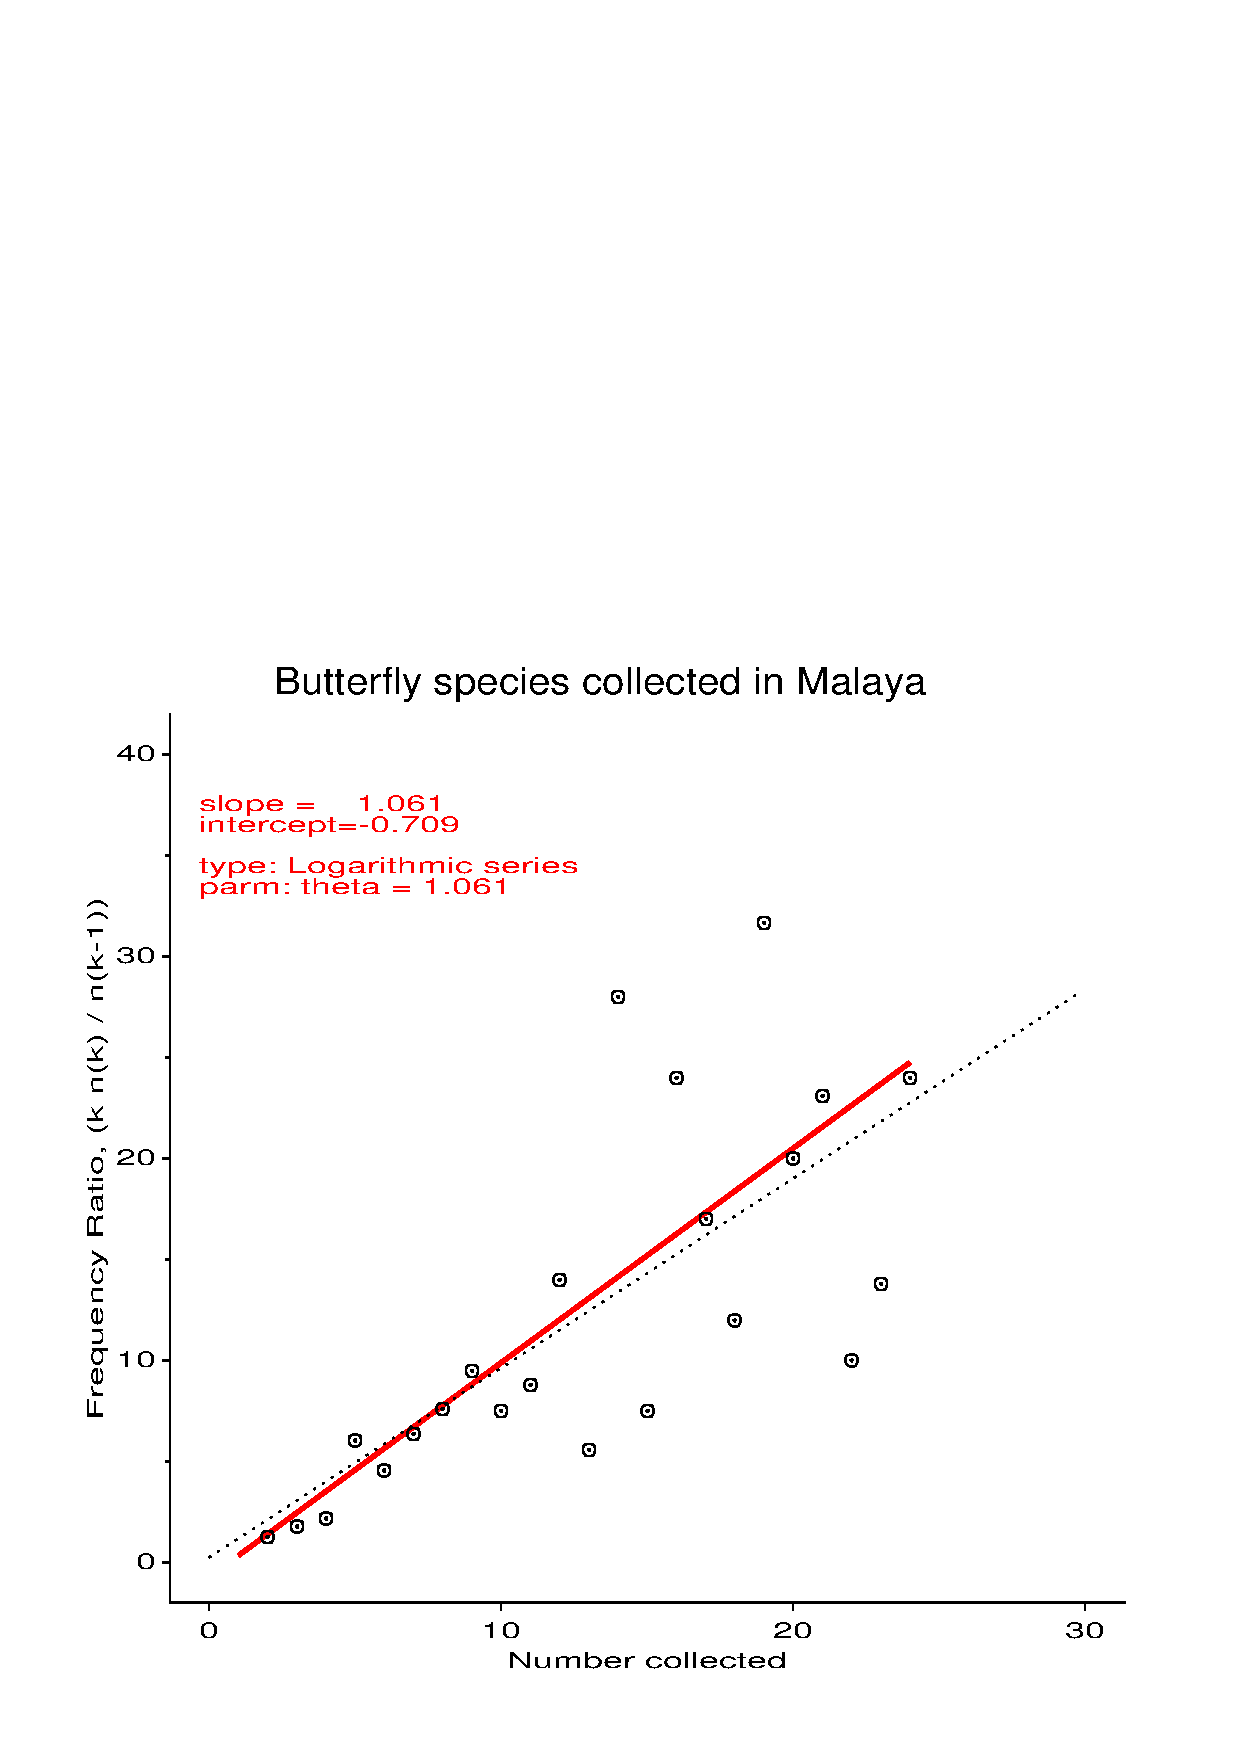
\includegraphics[width=1\linewidth]{orddemo3}\graphicsfile{ch2/fig/orddemo3.eps}{}
 \end{minipage}
 \hfill
 \begin{minipage}[c]{.33\linewidth}
  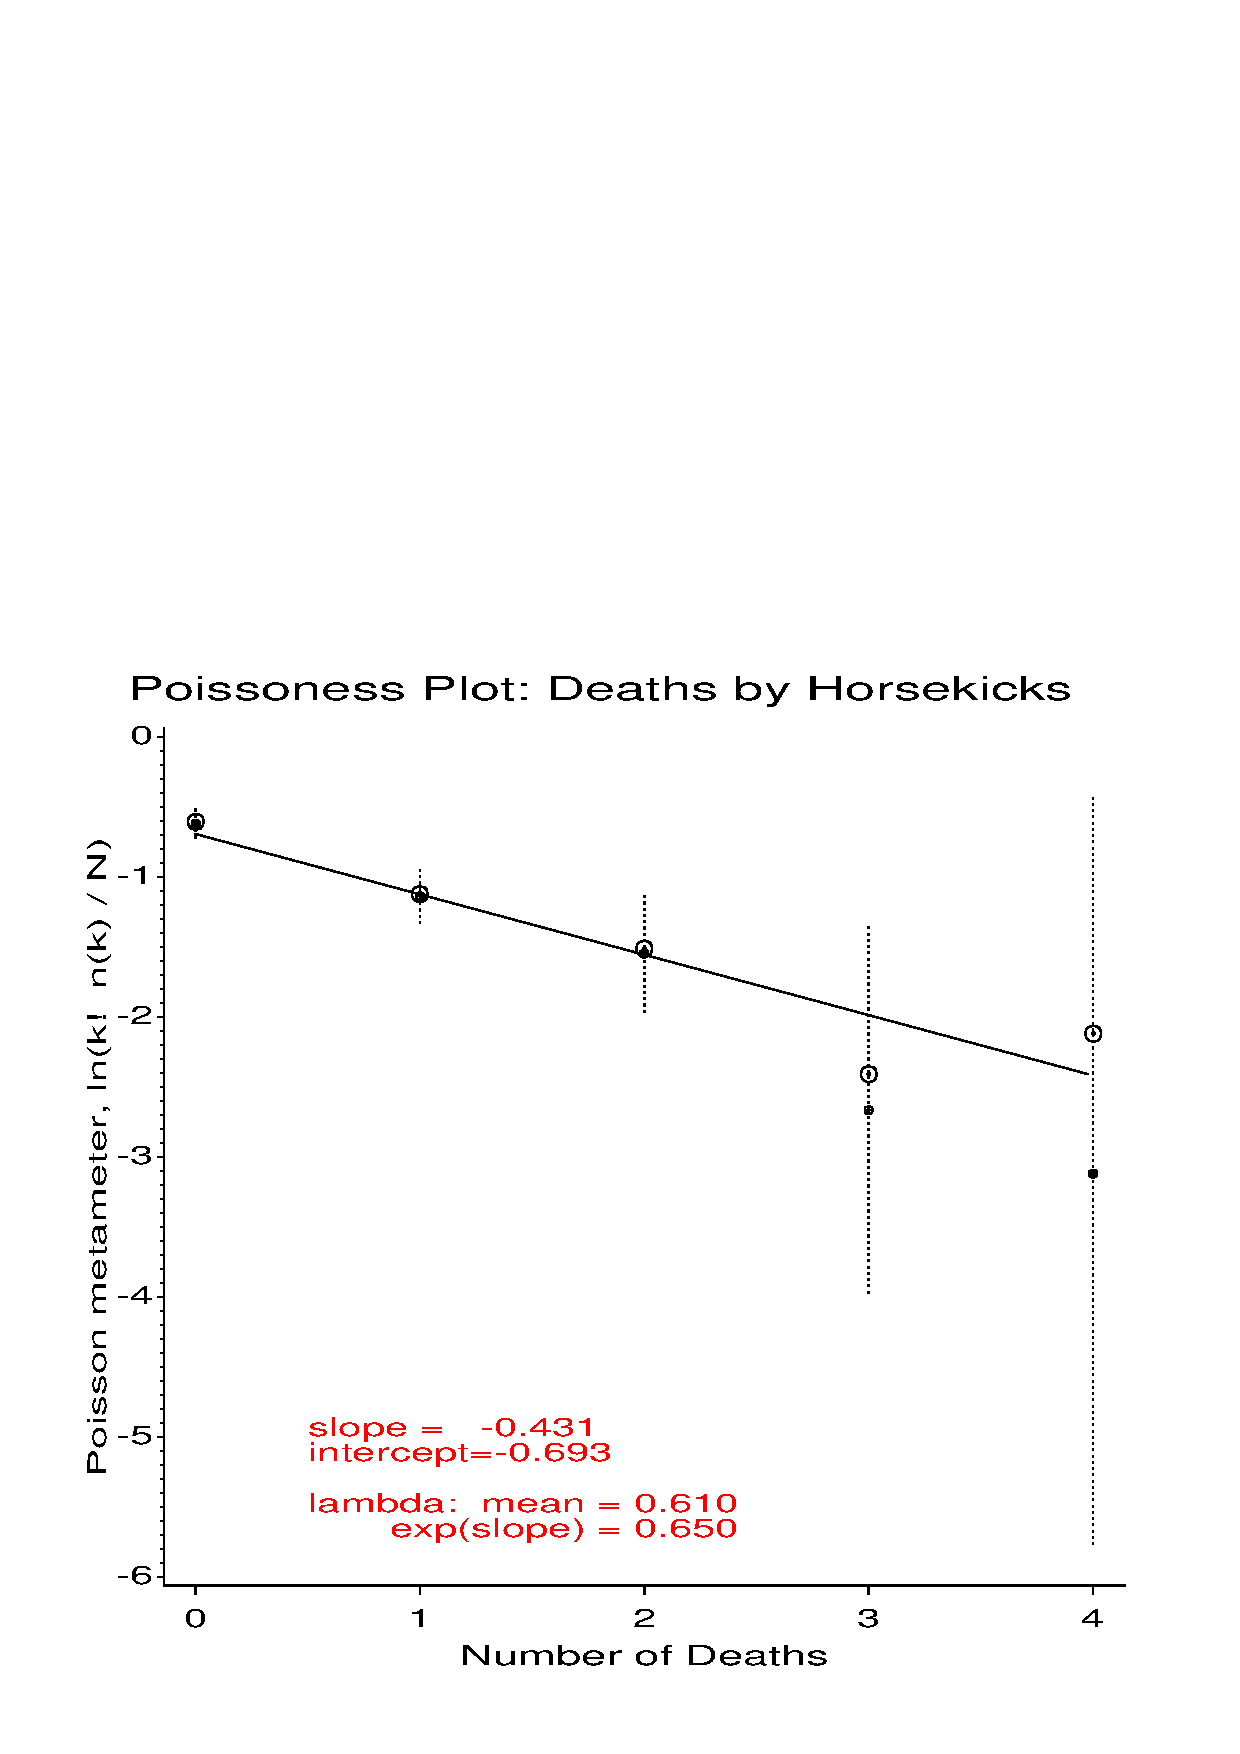
\includegraphics[width=1\linewidth]{poisdemo1}\graphicsfile{ch2/fig/poisdemo1.eps}{}
 \end{minipage}
\end{center}


\begin{quote}
{\Large
Categorical data consists of variables whose values comprise a set
of discrete categories.
Such data require different statistical and graphical methods
than commonly used for quantitative data.
The focus of this book is on visualization techniques and graphical
methods designed to reveal patterns of relationships among
categorical variables.
}
\end{quote}
\minitoc
\clearpage

\section{Data visualization and categorical data}
\epigraph{``Beauty is truth; truth, beauty.'' \\
  That is all ye know on Earth,
  all ye need to know.}{John Keats, \emph{Ode on a Grecian urn}}

``Data visualization'' is an approach to data analysis which focuses
on \emph{insighful graphical display}.  We may display the raw data, some
summary statistics, or some indicators of the quality or adequacy
of a fitted model.  The word ``insightful'' suggests that the goal
is (hopefully) to reveal some aspects of the data which might not
be perceived, appreciated, or absorbed by other means.  The overall
aims include both beauty and truth, though each of these are 
only as perceived by the beholder.

Methods for visualizing quantitative data have a long history
and are now widely used in both data analysis and in data presentation, and
in both popular and scientific media.
Graphical methods for categorical data,
however, have only recently developed, and are consequently
not as widely used.  The goal of this book is to show concretely how
data visualization may be usefully applied to categorical data.

``Categorical data'' means different things in different
contexts.  We introduce the topic in \secref{sec:intro-whatis}
with some examples illustrating
\begin{seriate}
\item types of categorical variables: binary, nominal, and ordinal,
\item data in case form vs.\ frequency form,
\item frequency data vs.\ count data,
\item univariate, bivariate, and multivariate data, and
\item the distinction between explanatory and response variables.
\end{seriate}

Methods for the analysis of categorical data also fall into two
quite different categories, described and illustrated in \secref{sec:intro-strat}: the simple randomization-based
methods typified by
the classical Pearson $\chi^2$, Fisher's exact test, and Cochran-Mantel-Haenszel
tests, and the model-based methods represented by
logistic regression, loglinear, and generalized linear models.
\chrange{ch:discrete}{ch:corresp}
are mostly related to the randomization-based methods; 
\chrange{ch:logistic}{ch:loglin}
illustrate the model-based methods.

In \secref{sec:intro-grmeth} we describe some important similarities
and 
differences between categorical data and
quantitative data, and discuss the implications of these differences for
visualization techniques.
\secref{sec:intro-visualize} outlines a strategy of data analysis
focused on visualization.

\renewcommand{\FileName}{whatis}

% slide template
\begin{frame}
  \frametitle{What is categorical data?}
  \begin{itemize}
	\item Simplest case: 1-way frequency distribution
      \begin{itemize*}
	  \item Unordered factor
	  \begin{flushright}
	  \includegraphics[width=.9\dispwidth]{fig/whatis1}
	  \end{flushright}
	  \item Ordered, quantitative factor
	  \begin{flushright}
	  \includegraphics[width=.9\dispwidth]{fig/whatis2}
	  \end{flushright}
	  \end{itemize*}
  \end{itemize}
\end{frame}

\begin{frame}
  \frametitle{What is categorical data?}
  \begin{itemize}
	\item Contingency tables ($2 \times 2 \times \dots$)
      \begin{itemize*}
	  \item Two-way
	  \begin{flushright}
	  \includegraphics[width=.8\dispwidth]{fig/whatis3}
	  \end{flushright}
	  \item Three-way
	  \begin{flushright}
	  \includegraphics[width=.9\dispwidth]{fig/whatis4}
	  \end{flushright}
	  \end{itemize*}
  \end{itemize}
\end{frame}

\begin{frame}
  \frametitle{What is categorical data?}
  \begin{itemize}
	\item Contingency tables (larger)
      \begin{itemize*}
	  \item Two-way
	  \begin{flushright}
	  \includegraphics[width=.7\dispwidth]{fig/whatis5}
	  \end{flushright}
	  \item Three-way
	  \begin{flushright}
	  \includegraphics[width=.8\dispwidth]{fig/whatis6}
	  \end{flushright}
	  \end{itemize*}
  \end{itemize}
\end{frame}


% two columns with text and figure
\begin{frame}
  \frametitle{Table and case-form}
  \begin{columns}[T]
    \begin{column}{.6\textwidth}
	  \begin{itemize}
		\item<1> The previous examples were shown in \alert{table} form
		  \begin{itemize*}
		    \item \# observations = \# cells in the table
			\item variables: factors + COUNT
		  \end{itemize*}
		\item<2> Each has an equivalent representation in \alert{case} form
		  \begin{itemize*}
		    \item \# observations = total COUNT
			\item variables: factors 
		  \end{itemize*}
		\item<3> Case form is required if there are continuous variables
	  \end{itemize}
    \end{column}
    \begin{column}{.4\textwidth}
    \includegraphics<1>[width=\textwidth,clip]{fig/whatis6}
    \includegraphics<2>[width=\textwidth,clip]{fig/whatis7}
    \includegraphics<3>[width=\textwidth,clip]{fig/whatis8}
    \end{column}
  \end{columns}
\end{frame}


\section{Strategies for categorical data analysis}\label{sec:intro-strat}
Methods of analysis for categorical data can be classified into two
broad categories:
those concerned with hypothesis testing \emph{per se}, and those concerned
with model building.

\subsection{Hypothesis testing approaches}
In many studies, the questions of substantive interest translate readily
into questions concerning hypotheses about association between variables.
If a non-zero association exists, we may wish to characterize the
strength of the association numerically and understand the pattern or
nature of the association.
For example, in \tabref{tab:berk220}, the question
``Is there evidence of gender-bias in admission to graduate school?''
may be expressed in terms of an association between gender and
admission status in a $2 \times 2$ \ctab\
of applicants classified by these two variables.
If so, we can assess the strength of the association by a variety of
measures, including the difference in proportions admitted for men
and women or the ratio of the odds of admission for men compared to
women, as described in \secref{sec:twoway-twobytwo}.

Similarly, in \tabref{tab:arthrit0}, questions about the efficacy of the
treatment for rheumatoid arthritis can be answered in terms of
hypotheses about the associations among the table variables
Treatment, Sex, and the Improvement categories.
Although the main concern might be focused on the overall association between
Treatment and Improvement, one would also wish to know if this association
is the same for men and women.  A stratified analysis (\secref{sec:twoway-strat}) controls for the effects of background
variables like Sex, and tests for \emph{homogeneity of association}
help determine if these associations are equal.

Questions involving tests of such hypotheses are answered most easily
using the randomization-based methods provided by \PROC{FREQ}.
These include the familiar Pearson chi-square,
the Cochran-Mantel-Haenszel test statistics, Fisher's exact test, and a wide variety of measures of strength of association.
These tests make minimal assumptions, principally requiring that subjects
or experimental units have been randomly assigned to the categories of
experimental factors.  The hypothesis testing approach is illustrated
in \chref{ch:twoway}--\ref{ch:corresp}, though the emphasis is on graphical
methods which help to understand the nature of association between
variables.
\begin{Example}[haireye0]{Hair color and eye color}
Two graphical methods related to the hypothesis testing approach
are shown in \figref{fig:haireye0}.
The data concern the relationship between hair color and eye color
in a sample of nearly 600 students (see \tabref{tab:hairdat} and \datref{dat:haireye}).
The standard analysis with \PROC{FREQ} gives a 
Pearson \(\chi^2\) of 138.3 with nine degrees of freedom,
indicating substantial departure from independence.  How do we
understand the {\emph{nature}} of this association between hair
and eye color?

%% two subfig side-by-side
\begin{figure}[htb]
 \begin{minipage}[c]{.49\linewidth}
  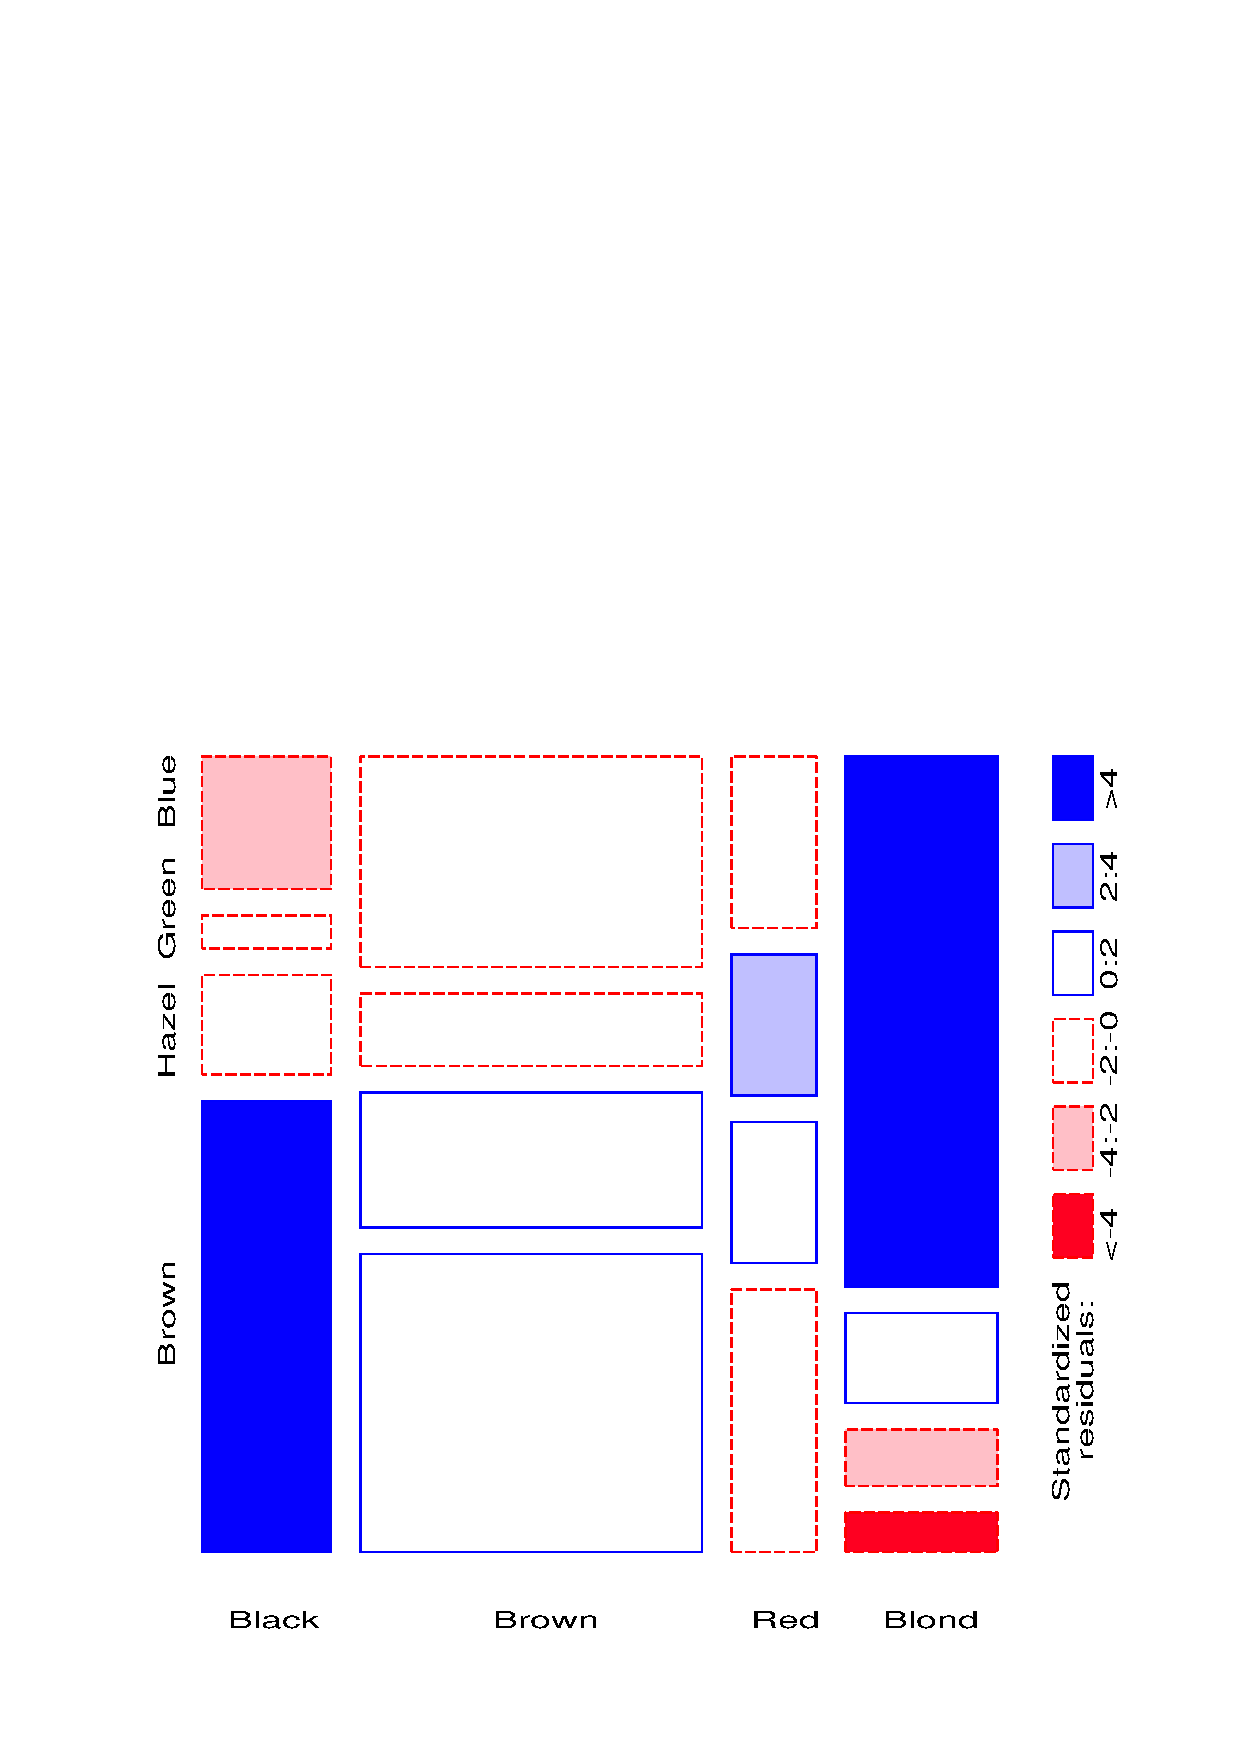
\includegraphics[width=1\linewidth,clip]{ch4/fig/mosaic34}
 \end{minipage}%
 \hfill
 \begin{minipage}[c]{.49\linewidth}
  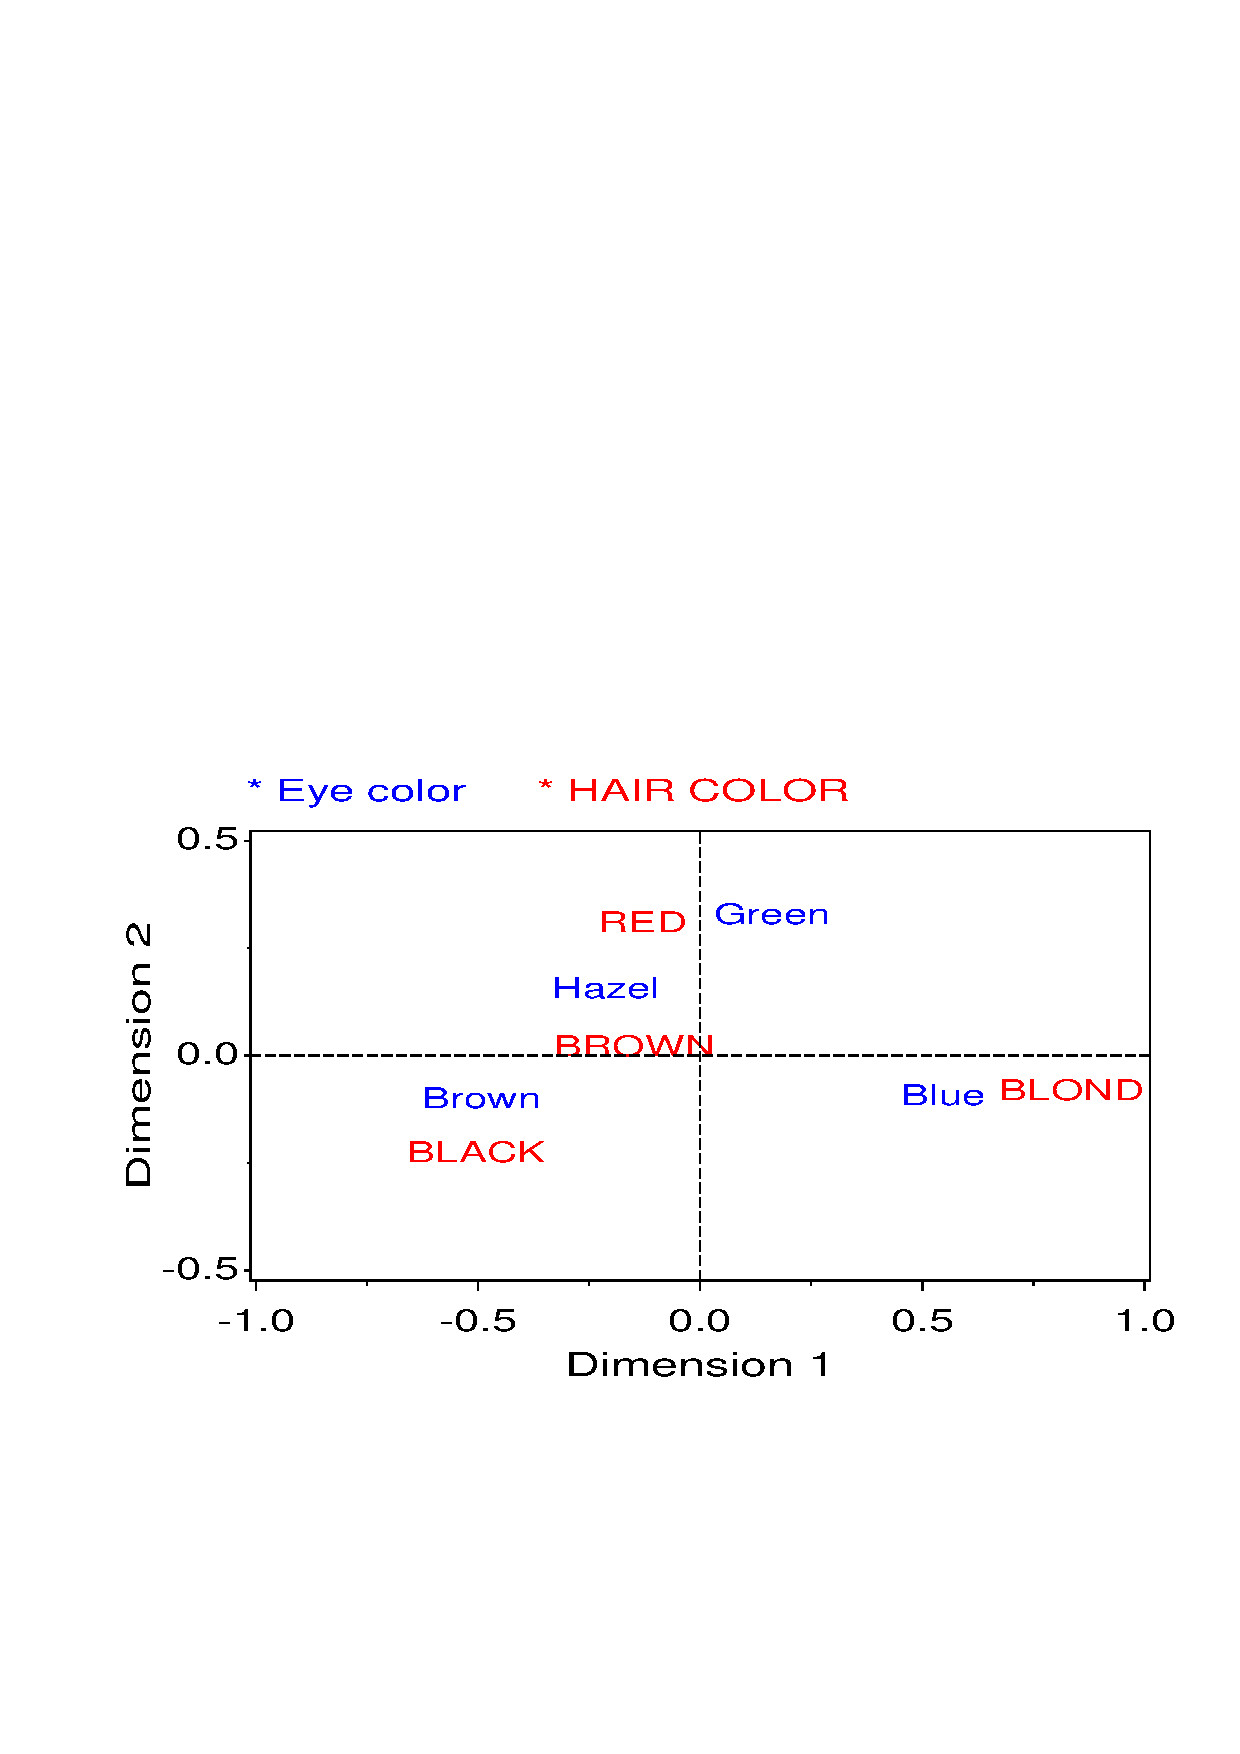
\includegraphics[width=1\linewidth,clip]{ch5/fig/corresp3}
 \end{minipage}
 \caption[Graphical displays for hair color and eye color data]{Graphical displays for hair color and eye color data. Left: mosaic display; right:  correspondence analysis 2D solution.}\label{fig:haireye0}
\end{figure}

The left panel of \figref{fig:haireye0} is a mosaic display
(\chref{ch:mosaic}), constructed so that the size of each rectangle
is proportional to the observed cell frequency. The shading
reflects the cell contribution to the \(\chi^2\) statistic---shades of blue
when the observed frequency is substantially greater than the 
expected frequency under independence, shades of red when the observed freqency
is substantially less, as shown in the legend.

The right panel of this figure shows the results of 
a \CA\ (\chref{ch:corresp}), where the deviations of the hair color and eye
color points from the origin accounts for as much of the \(\chi^2\)
as possible in two dimensions.

We observe that both the hair colors and the eye colors
are ordered from dark to light in the mosaic display and along
Dimension 1 in the \CA\ plot.  The deviations between observed
and expected frequencies have an opposite-corner pattern in the
mosaic display, except for the combination of red hair and green
eyes, which also stand out as the largest values on Dimension 2
in the \CA\ plot.
Displays such as these provide a means to understand \emph{how}
the variables are related.
\end{Example}
 
\subsection{Model building approaches}
In other situations, model-based methods provide tests of equivalent
hypotheses about associations, but (at the cost of additional assumptions)
offer additional advantanges
not provided by the simpler hypotheses-testing approaches.
As in the analysis of quantitative data, linear statistical models
relate the expected value of a response to a linear function of
the table variables, and also assume that residuals or deviations
from the model follow a known parametric form.

For a dichotomous response variable, for example, it is convenient to
construct a model relating a function of the probability, $\pi$,
of one event to a linear combination of the explanatory variables.
Logistic regression uses the logit function,
\begin{equation*}
 \logit ( \pi ) = \log_e \frac { \pi } {1 - \pi}
\end{equation*}
which may be interpreted as the log odds of the given event.

Statistical inferences from model-based methods also provide tests of
hypotheses, but they provide estimates of parameters in the model
and associated confidence intervals and prediction intervals for the 
response as well.  A particular advantage of the logit represention
in the logistic regression model is that estimates of odds ratios
(\secref{sec:twoway-odds})
may be obtained directly from the parameter estimates.

\begin{Example}[nasa0]{Challenger disaster}
\ixd{Challenger disaster|(}
To illustrate, the graph in \figref{fig:nasa1} is based on
a logistic regression model predicting the probability of a
failure in one of the O-ring seals used in the NASA space shuttles
prior to the disasterous launch of the 
\emph{Challenger} in January, 1986.  The explanatory variable is the ambient temperature at the time of the flight.
The sad story behind these data, and the lessons to be learned for
graphical data display are related in \exref{ex:nasa}.
\begin{figure}[htb]
  \centering
  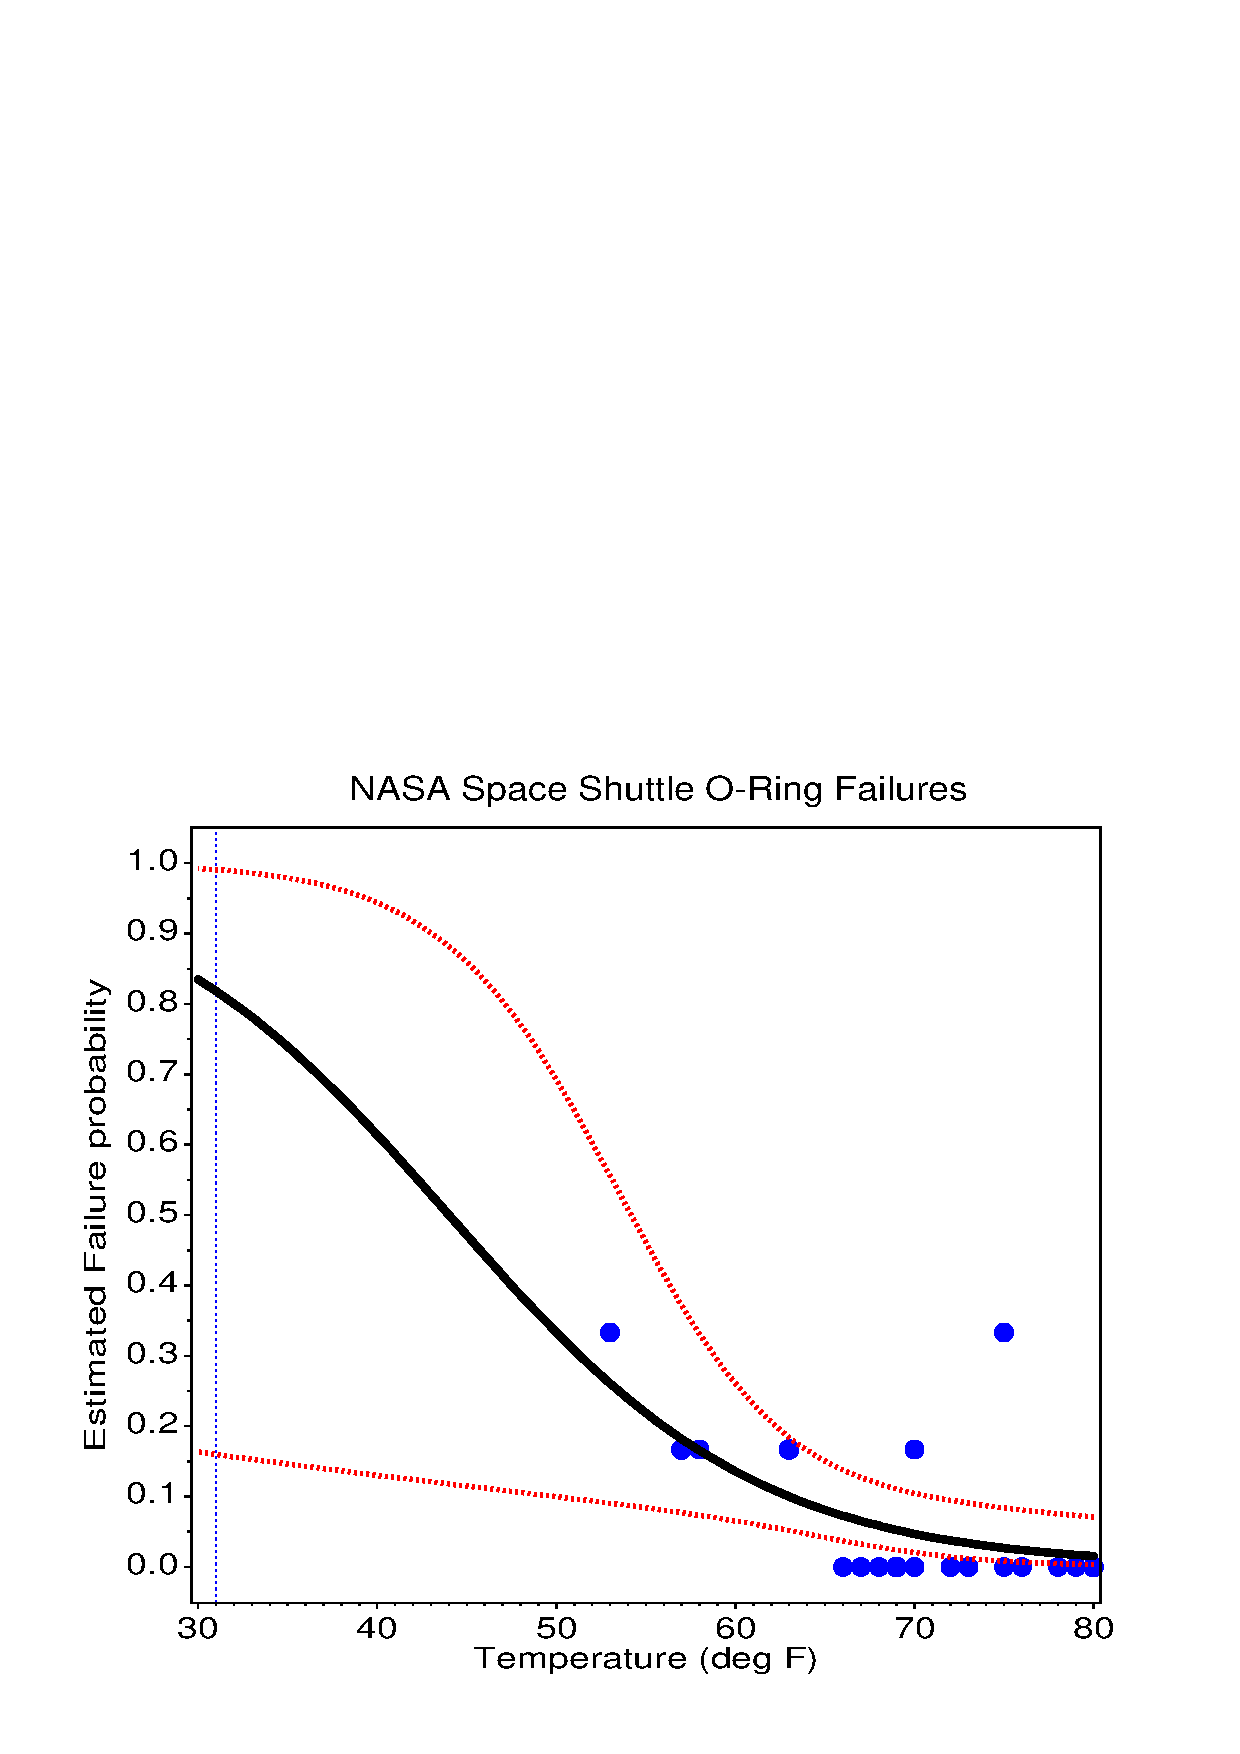
\includegraphics[scale=.6]{ch6/fig/nasa}
  \caption{NASA Space Shuttle 
  O-ring Failure, Observed and Predicted probabilities}\label{fig:nasa1}
\end{figure}

Here, we simply note that the fitted model, shown by the solid line in
\figref{fig:nasa1}, corresponds to the prediction equation
(with standard errors shown in parentheses),
\begin{equation*}
 \logit ( \mbox{Failure} ) =  \cwe{5.09}{3.06} - \cwe{0.116}{0.047} \mbox{ Temp} 
 \end{equation*}%
An hypothesis test that failure probability is unassociated with temperature
is equivalent to the test that the coefficient for temperature in this
model equals 0; this test has a $p$-value of 0.014, convincing evidence
for rejection.
The parameter estimate for temperature, $-0.116$, however, gives more information.  Each \degree{1} increase in temperature decreases the log odds
of failure by 0.116, with 95\% confidence interval ($-0.208$, $-0.0235$).  The equivalent odds ratio is $\exp(-0.116) = 0.891$ (0.812--0.977).
Equivalently, a \degree{10} \emph{decrease} in temperature corresponds to
an odds ratio of a failure of 
$\exp(10 \times 0.116) = 3.18$, more than tripling the odds of a failure.
 
When the \emph{Challenger} was launched, the temperature was only \degree{31}.
The dashed lines in \figref{fig:nasa1} show 95\% prediction intervals
for failure probability.  All previous shuttles (shown by the points
in the figure) had been launched at much warmer temperatures, so the
prediction interval (the dashed vertical line)
at \degree{31} represents a considerable extrapolation
beyond the available data.  Nonetheless, the model building approach
does provide such predictions along with measures of their uncertainty.
\figref{fig:nasa1} is a graph
that might have saved lives.
\ixd{Challenger disaster|)}
\end{Example}

An additional advantage of the model-building approach is that it often
provides greater flexibility and allows more detailed or specialized
descriptions of the relations among variables to be tested.
For instance, in square, two-way tables such as those classifying
the occupations of fathers and sons, or attitudes of husbands and wives,
specialized models dealing with symmetry or forms of lack of symmetry
may be fit and tested.  Such models are usually of much greater
substantive interest than the hypothesis of general association.
Similarly, specialized models for ordinal variables allow more detailed
tests of the nature of association to be examined.
\chref{ch:mosaic} and
\chrange{ch:logistic}{ch:loglin} illustrate many forms of these
specialized models.


%\subsection{Exploratory vs.\ confirmatory analysis}
%A related distinction is that between exploratory and confirmatory
%methods of data analysis.
 


%\section{Sampling models for categorical data}

\section{Graphical methods for categorical data}\label{sec:intro-grmeth}
\epigraph{You can see a lot, just by looking}{Yogi Berra}

The graphical methods for categorical data described in this book
are in some cases straightforward adaptations of more familiar
visualization techniques developed for quantitative data.
The graphical principles and strategies, and the relations between
the visualization approach and traditional statistical methods
are described in \SSSG, Chapter 1, and \cite{Cleveland:VisData}.
Another perspective on visual data display is presented in \secref{sec:intro-goals}.
However, the discrete nature of categorical data implies that
some familiar graphic methods need to be adapted, while in other
cases we require a new graphic metaphor for data display.
These issues are illustrated in \secref{sec:intro-catdata}.

\subsection{Goals and design principles for visual data display}\label{sec:intro-goals}

Designing good graphics is surely an art, but as surely, it is
one that ought to be informed by science.
In constructing a graph, quantitative and qualitative information is
encoded by visual features, such as position, size, texture, symbols
and color. This translation is reversed when a person studies a
graph. The representation of numerical magnitude and categorical
grouping, and the aperception of patterns and their \emph{meaning} must be extracted from the visual display.  

There are many views of graphs, of graphical perception, and of
the roles of data visualization in discovering and communicating
information.
On the one hand, one may regard a graphical display as a ``stimulus'' --
a package of information to be conveyed to an idealized observer.
From this perspective certain questions are of interest:  which
form or graphic aspect promotes greater accuracy or speed of judgment
(for a particular task or question)?  What aspects lead to greatest
memorability or impact? 
Cleveland \citep{ClevelandMcGill:84b,ClevelandMcGill:85,Cleveland:93:JCGS},
Lewandowsky and
Spence
\citep{LewandowskySpence:89,Spence:90} have made important contributions to our understanding of
these aspects of graphical display.

An alternative view regards a graphical display as an act
of communication---like a narrative, or even a poetic text or work of art. 
This perspective places the greatest emphasis on the desired
communication goal, and judges the effectiveness of a graphical
display in how well that goal is achieved.
\citet{Kosslyn:85,Kosslyn:89} and \citet{Tufte:83,Tufte:90,Tufte:97}
have articulated this perspective most clearly.

In this view,
an effective graphical display, like good writing, requires an
understanding of its purpose---what aspects of the data are to be
communicated to the viewer.  In writing we communicate most
effectively when we know our audience and tailor the message
appropriately. So too, we may construct a graph in different ways to
use ourselves, to present at a conference or meeting of our
colleagues, or to publish in a research report, or a communication
to a general audience
\cite[Ch. 1]{Friendly:91}.

\figref{fig:datadisp}
shows one organization of visualization methods in terms
of the primary use or intended communication goal,
the functional presentation goal, and suggested corresponding
design principles.
\begin{figure}[htbp]
  \centering 
  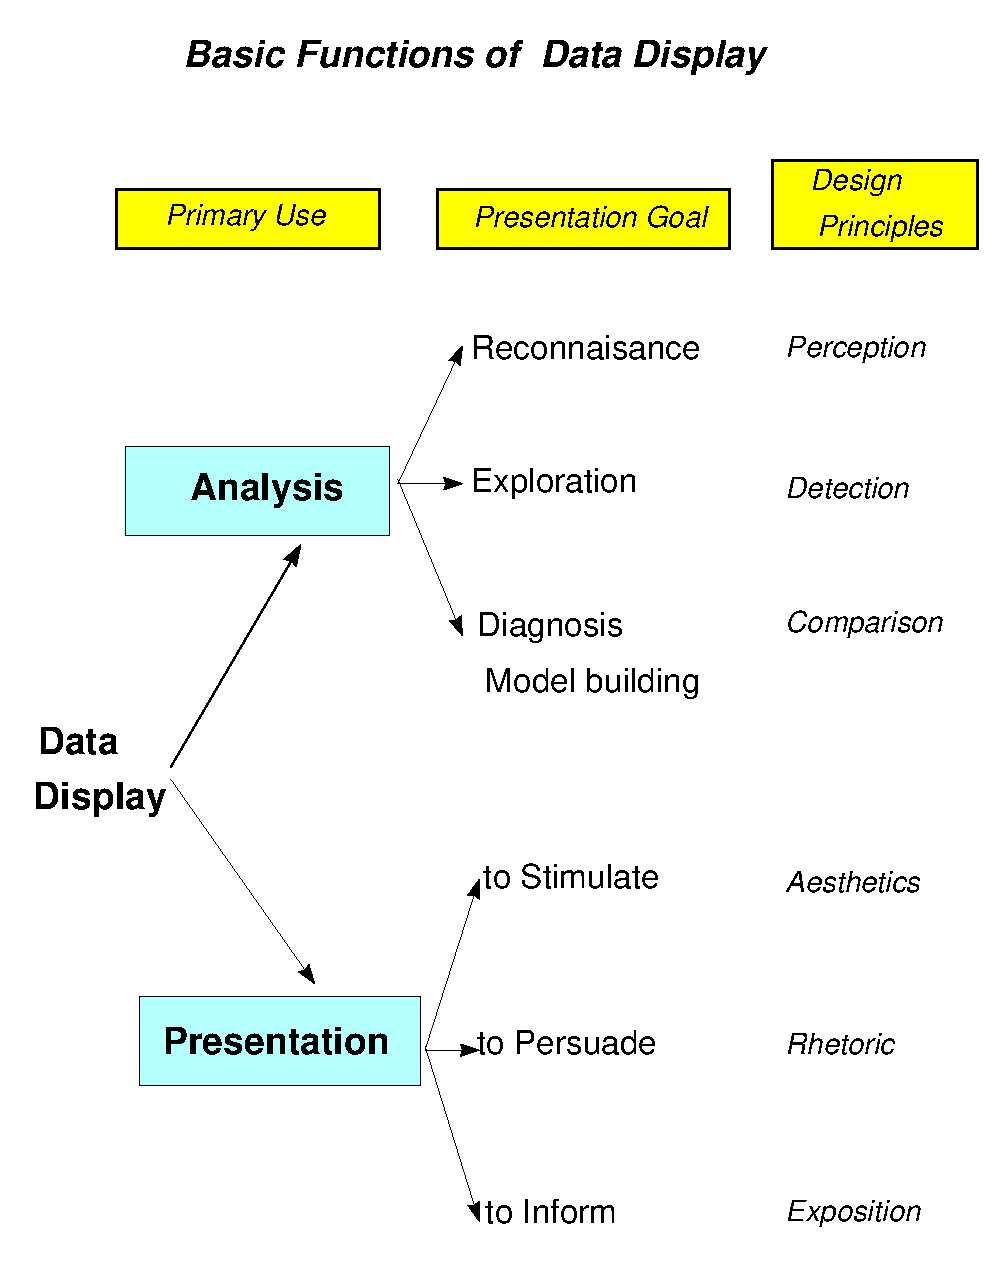
\includegraphics[scale=.8]{ch1/fig/datadisp}
  \caption[Basic functions of data display]{A taxonomy of the basic functions of data display by intended use and presentation goal}\label{fig:datadisp}
\end{figure}

The first distinction identifies \boldital{Analysis} or 
\boldital{Presentation} as the primary
communication goal of a data graphic
(with the understanding that a given graph may serve both purposes---or,
sadly, neither).

\subsubsection{Analysis graphs}
Graphs used for data analysis should clearly show the data, but they
should also ``force us to notice what we never
expected to see''
\cite[p. vi]{Tukey:77}.

Among graphical methods designed to help study or understand
a body of data, we may distinguish those designed for different
purposes.  As suggested in \figref{fig:datadisp}, each presentation goal
is associated with somewhat different design principles.
\begin{itemize}
\item \boldital{reconnaissance}---a preliminary examination, or an overview of a possibly complex terrain.
For this goal, we may be willing to sacrifice detail for a wider field of
view.
With a large, multi-way contingency table, for example, we might wish to
examine the collection of one-way and two-way marginal subtables
visually.  
\item \boldital{exploration}---graphs designed to help detect patterns or unusual
circumstances, or to suggest hypotheses, analyses or models.
For a binary response and a number of categorical or quantitative predictors,
a collection of smoothed plots of the response against each predictor
may suggest important variables to be included in a model,
extreme observations which should be examined, etc.
\item \boldital{diagnosis}---graphs designed to summarize or critique
a numerical statistical summary.
\end{itemize}

\subsubsection{Presentation graphs}
Presentation graphics have different goals as well.
We may wish to stimulate, or to persuade, or simply to inform.
As in writing, it is usually a good idea to know what it is you
want to say with a graph, and tailor its message to that goal.

It is often the case that a graph originally prepared as an aid
to data analysis can be transformed to one intended for presentation
by simple re-design.
Sometimes this entails removing detail useful for the analyst
but which may be detract from the major message;
sometimes this may involve adding titles or annotation to make the
message more immediately apparent.
In still other cases, we may decide to change the graphic format
to make visual comparisons easier for the intended audience.

For example, \figref{fig:glogist00} shows two views of the results
of fitting a logistic regression model to the arthritis treatment
data (described in \secref{sec:logist-qual}).
The left panel shows the observed (points) and predicted probabilities of
improvement ($\pm 1$ standard error, giving approximate 67\%
confidence intervals) in the form of a line graph.
The right panel shows a possible re-design of this graph for presentation
purposes.
%% two subfig side-by-side
\begin{figure}[htb]
 \begin{minipage}[c]{.49\linewidth}
  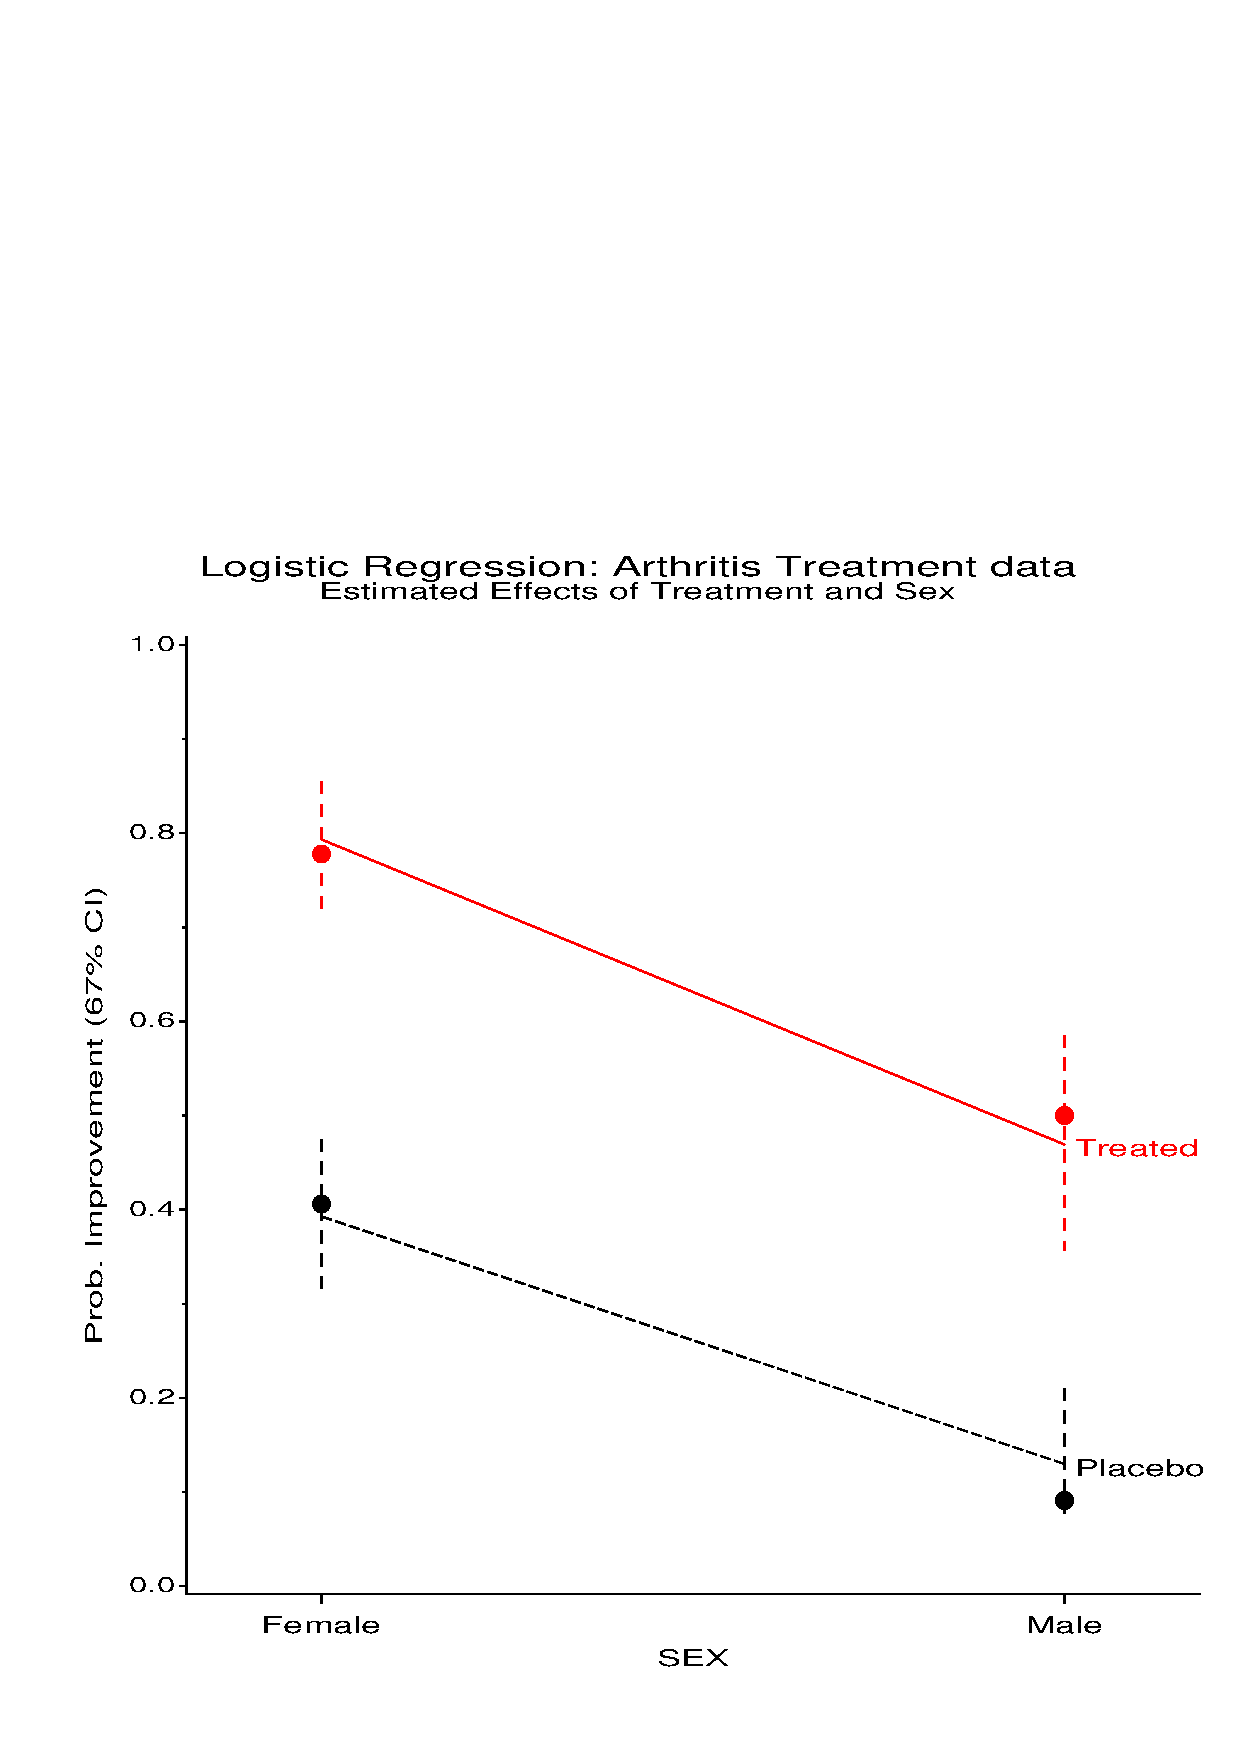
\includegraphics[width=1\linewidth]{ch6/fig/glogist11}
 \end{minipage}%
 \hfill
 \begin{minipage}[c]{.49\linewidth}
  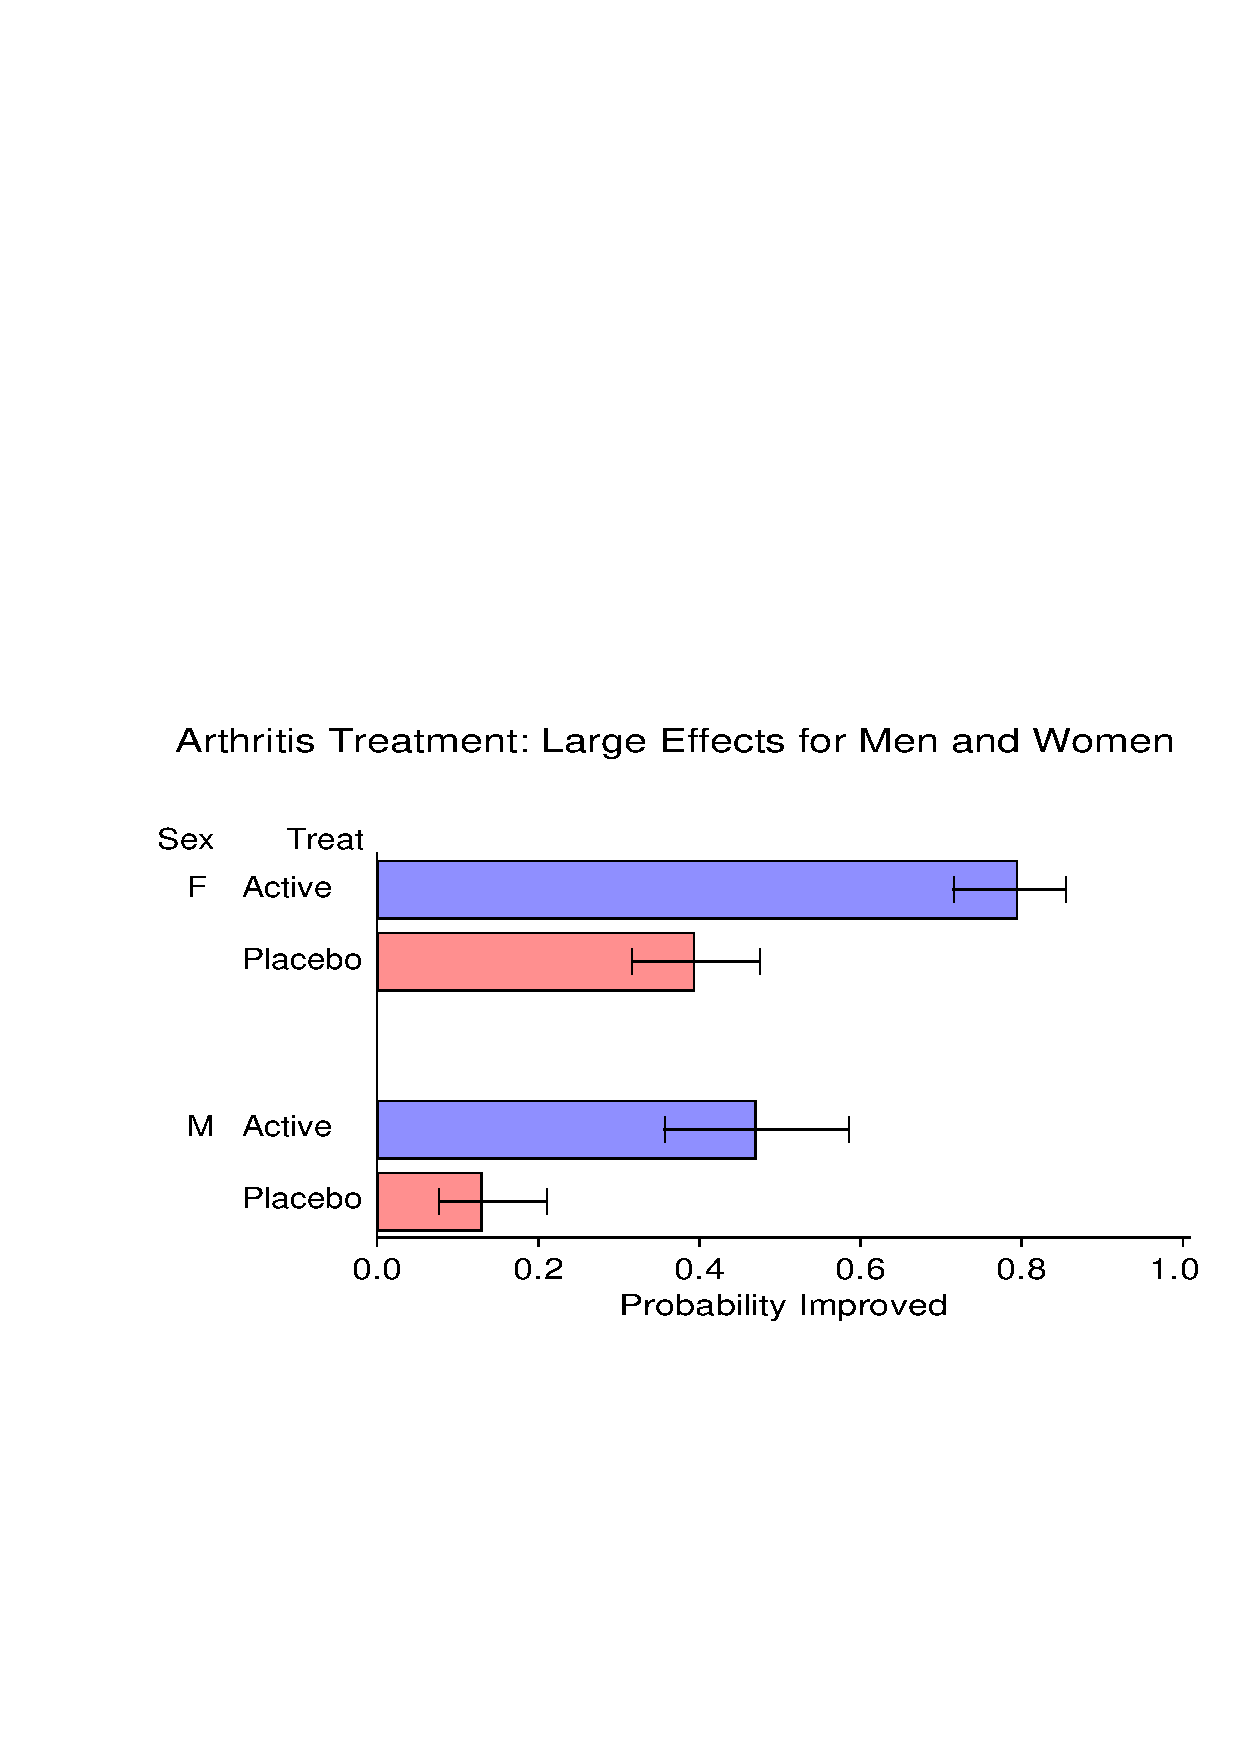
\includegraphics[width=1\linewidth,clip]{ch1/fig/glogist00}
 \end{minipage}
 \caption[Two graphical displays for arthritis treatment data]{Two graphical displays for arthritis treatment data. Left: initial analysis graph; right: re-design for presentation.}\label{fig:glogist00}
\end{figure}

The line graph might be preferred for analysis purposes, because it
shows
\begin{seriate}
\item the observed and fitted probabilities are quite similar,
\item there is a large effect of both treatment and sex, and
\item the effect of treatment is about the same for both men and women.
\end{seriate}
The presentation version contains the same predicted probabilities and error
bars as the original graph, but omits the observed probabilities
for simplicity.
The title explicitly
announces the conclusion to be drawn from the graph.



\subsection{Categorical data require different graphical methods}\label{sec:intro-catdata}

We will see in Chapters 6--7 that statistical models for discrete
response data and for frequency 
data are close analogs of the linear regression and ANOVA models
used for quantitative data.
These analogies suggest that the graphical methods
commonly used for quantitative data may be adapted directly to
categorical data.

Happily, it turns out that many of the analysis graphs and diagnostic
displays (e.g., influence plots, added variable and partial residual
plots, etc.)
which have become common adjuncts in the analysis of
quantitative data have been extended to generalized linear models
including logistic regression and \loglin\ models.

Unhappily, the familiar techniques for displaying raw data are
often disappointing when applied to categorical data.
The simple \scat, for example, is widely used to show
the relation between
quantitative response and predictors, together with the fitted linear
model.
For the arthritis data in case form (\datref{dat:arthrit})
the analogous plot for a logistic regression model
(predicting Pr(Some or Marked) improvement from Age) shown in the
left panel of \figref{fig:logist1c0}, is, well,  underwhelming.
First, the response, Improve, takes on only the values 0 and 1,
and Age (in years) is also discrete, so many points overplot
in this graph.%
\footnote{Only 51 distinct points are shown for the 84 observations.}
Second, although this graph is enhanced with the curve of predicted
probabilities under the fitted model (solid line) and 95\% confidence
bands (dashed lines), it is hard to appreciate how the data points
relate to the fitted model.  (Can you see that the probability of
improvement increases with age?)
%% two subfig side-by-side
\begin{figure}[htb]
 \begin{minipage}[c]{.49\linewidth}
  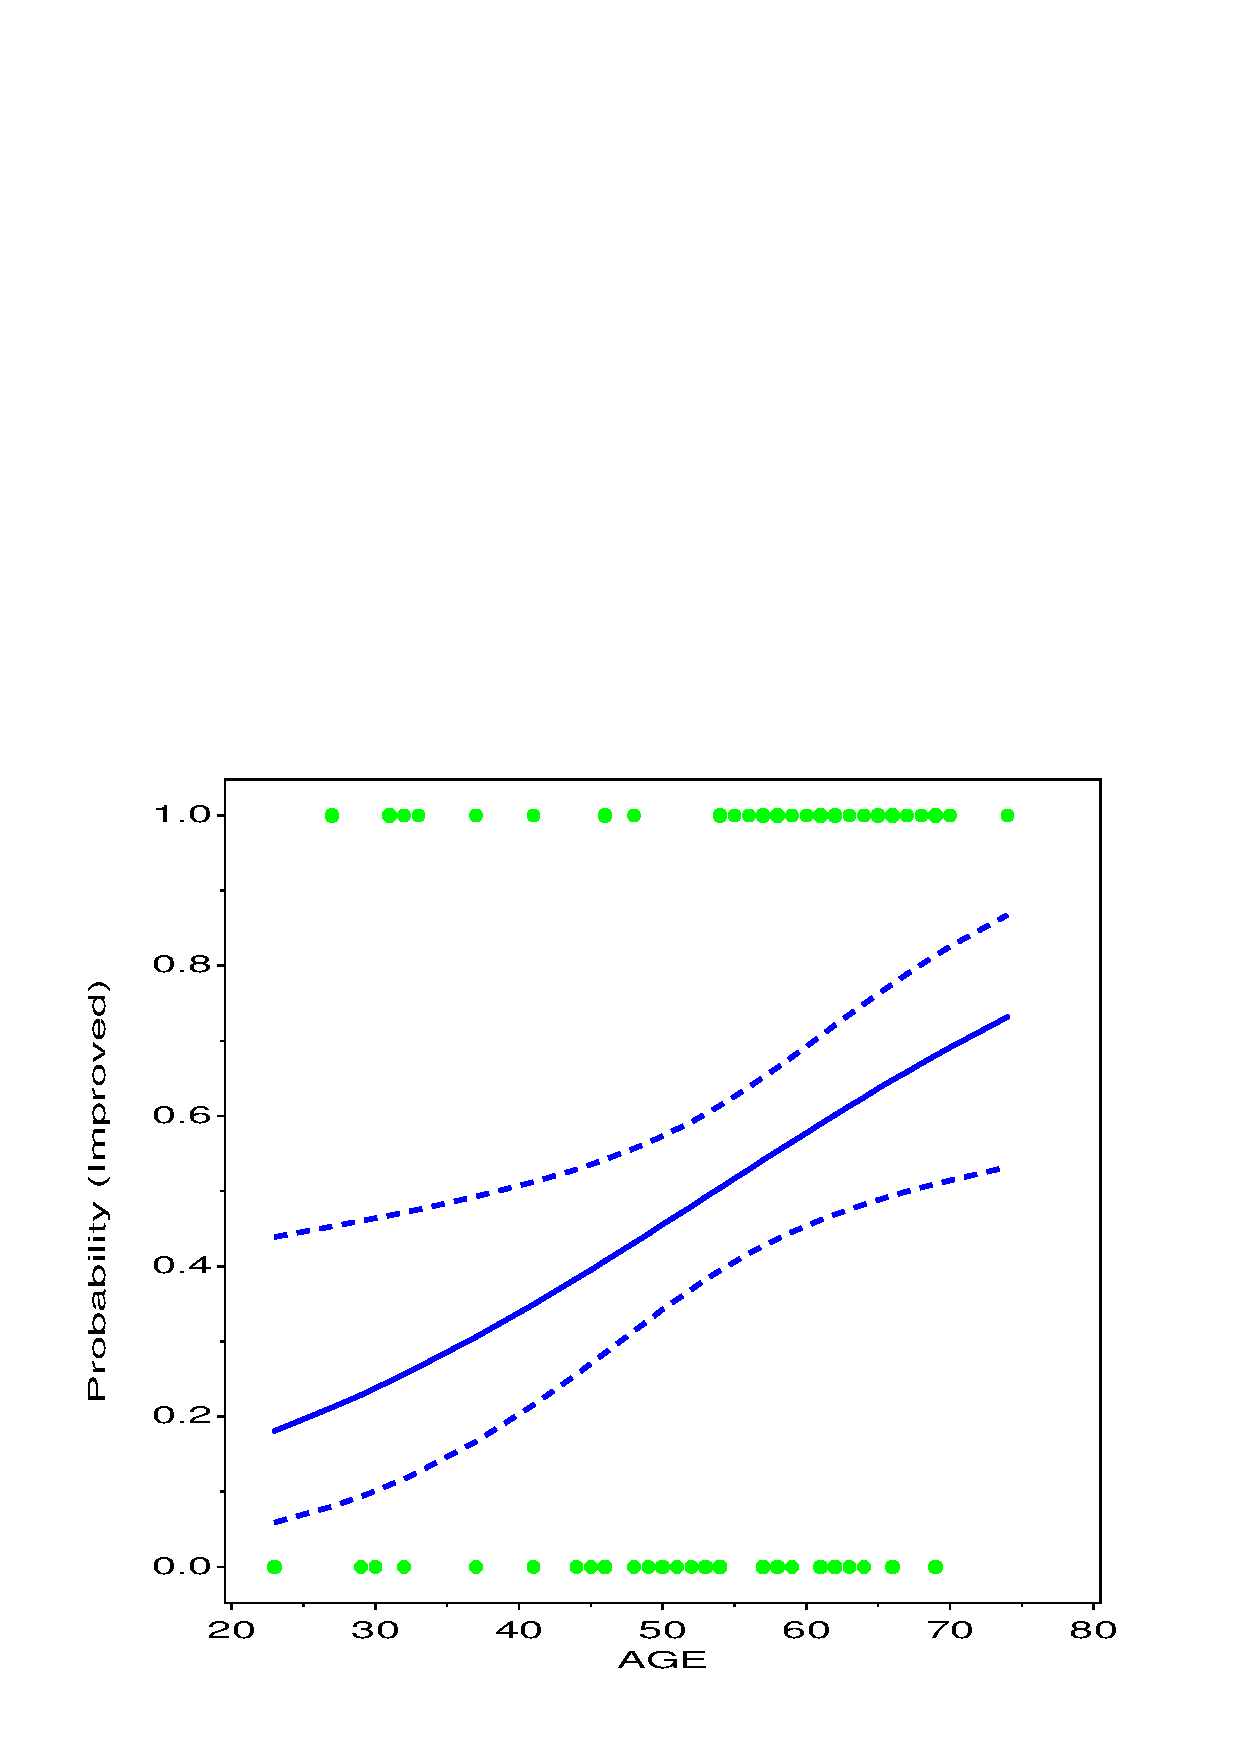
\includegraphics[width=1\linewidth,clip]{ch1/fig/logist1c0}
 \end{minipage}%
 \hfill
 \begin{minipage}[c]{.49\linewidth}
  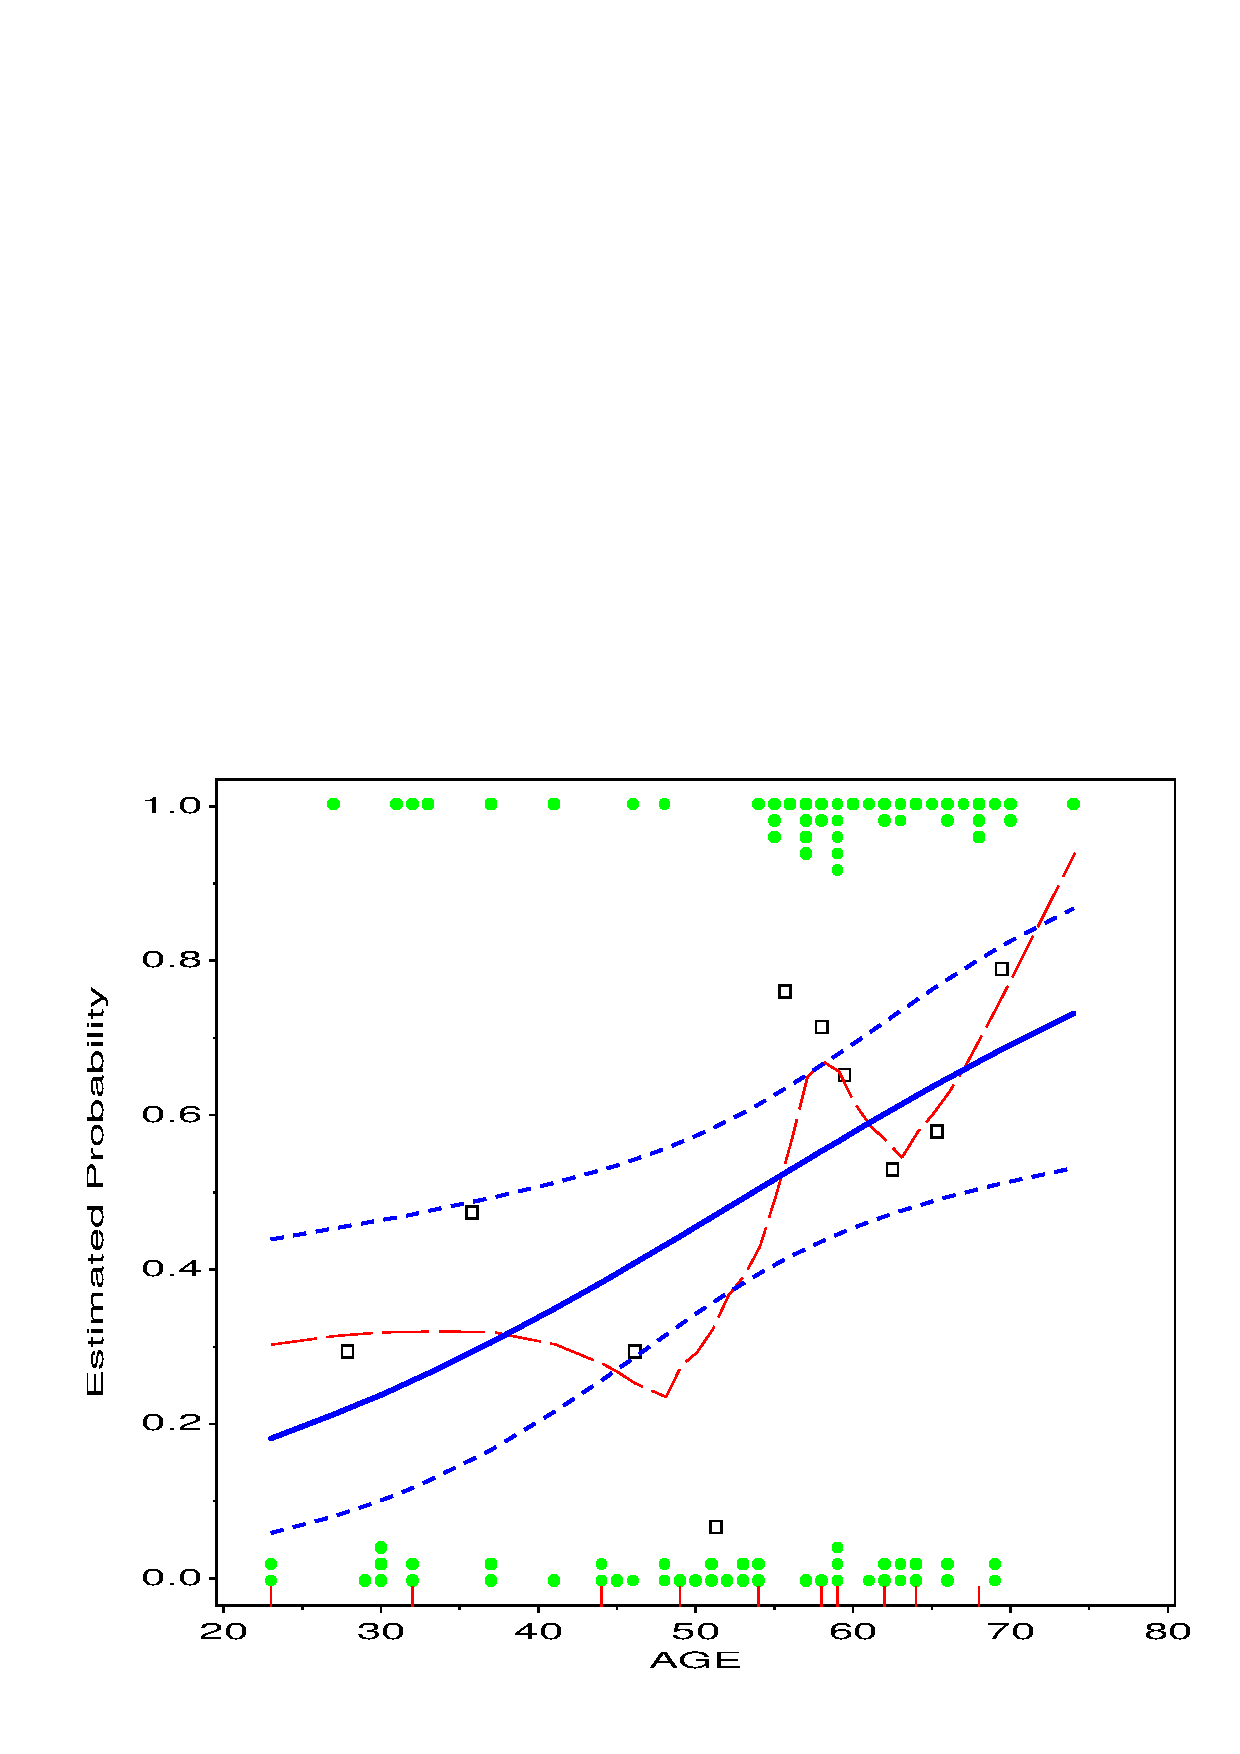
\includegraphics[width=1\linewidth,clip]{ch6/fig/logoddt2}
 \end{minipage}
 \caption[Graphical displays for Arthritis treatment data]{Graphical displays for Arthritis treatment data. Left: raw data
 with logistic regression on age; right: stacked raw data, logistic regression, and smoothed lowess curve.}\label{fig:logist1c0}
\end{figure}


These problems may be reduced to some degree by smoothing and by
jiggling the points to avoid overplotting.
The right panel of \figref{fig:logist1c0} shows a modest improvement.
Here, the raw observations were offset by stacking down from 1 and up
from 0 wherever duplicate observations occurred.
In addition, the observations were grouped into tenths by age; the lower
boundaries of the age categories are shown by the tick marks on the horizontal
scale.  The proportion of Improved responses in each age group is then
plotted (squares), and a non-parametric (lowess) smoothed curve is added
to the plot.
Although the smoothed curve is somewhat jagged, we now have a clearer
visual impression that the probability of improvement increases with age,
and we can see the large number of 1 responses among older people.

In \figref{fig:logist1c0} the quantitative variable Age supports
the use of the \scat\ as the graphic format for visual display. 
A more essential difference between quantitative data and categorical
data arises when all variables are categorical, as in a \ctab\
like \tabref{tab:arthrit0}.   Then, we find that a different visual
representation is more natural and useful
\citep{Friendly:95,Friendly:97}.  

For quantitative data, magnitude can
be represented by length (in a bar chart) or by position along a
scale (dotplots, scatterplots).  When the data are purely categorical,
design principles of perception, detection, and comparison
\citep{Friendly:99} suggest that frequencies are most usefully
represented as areas.  In spite of the fact that
(in magnitude estimation tasks) judgments of
area are known to be less accurate than those of length
(e.g., \citet{ClevelandMcGill:84b}), there
are two fundamental reasons why area is a preferred visual representation
for count data:
\begin{itemize}
\item multiplicative relations of probabilities and expected frequencies
translate readily into height and width of rectangles, whose area then
depicts a cell value.

\item a concrete, physical model for categorical data \citep{Friendly:95}
based on count $\sim$ area 
yields a surprising range of correct, but novel
interpretations for statistical principles (maximum likelihood),
estimation techniques (iterative proportional fitting, Newton--Raphson)
and statistical concepts (power, why components of likelihood-ratio $G^2$ can be
negative).
\end{itemize}

\ix{sieve diagram|(}
The first point is illustrated in \figref{fig:sievebrk1},
a sieve diagram (\secref{sec:twoway-sieve})
for the Berkeley admissions data, broken down by department.
In this display, each box has a height proportional to the marginal total
for the corresponding department and width proportional to the column
marginal total, so the area is proportional to the expected frequency
under independence.  The observed frequency in each cell is shown
by the number of cross-ruled boxes, so departures from independence
are shown visually as variations in shading density.
\begin{figure}[htb]
  \centering
  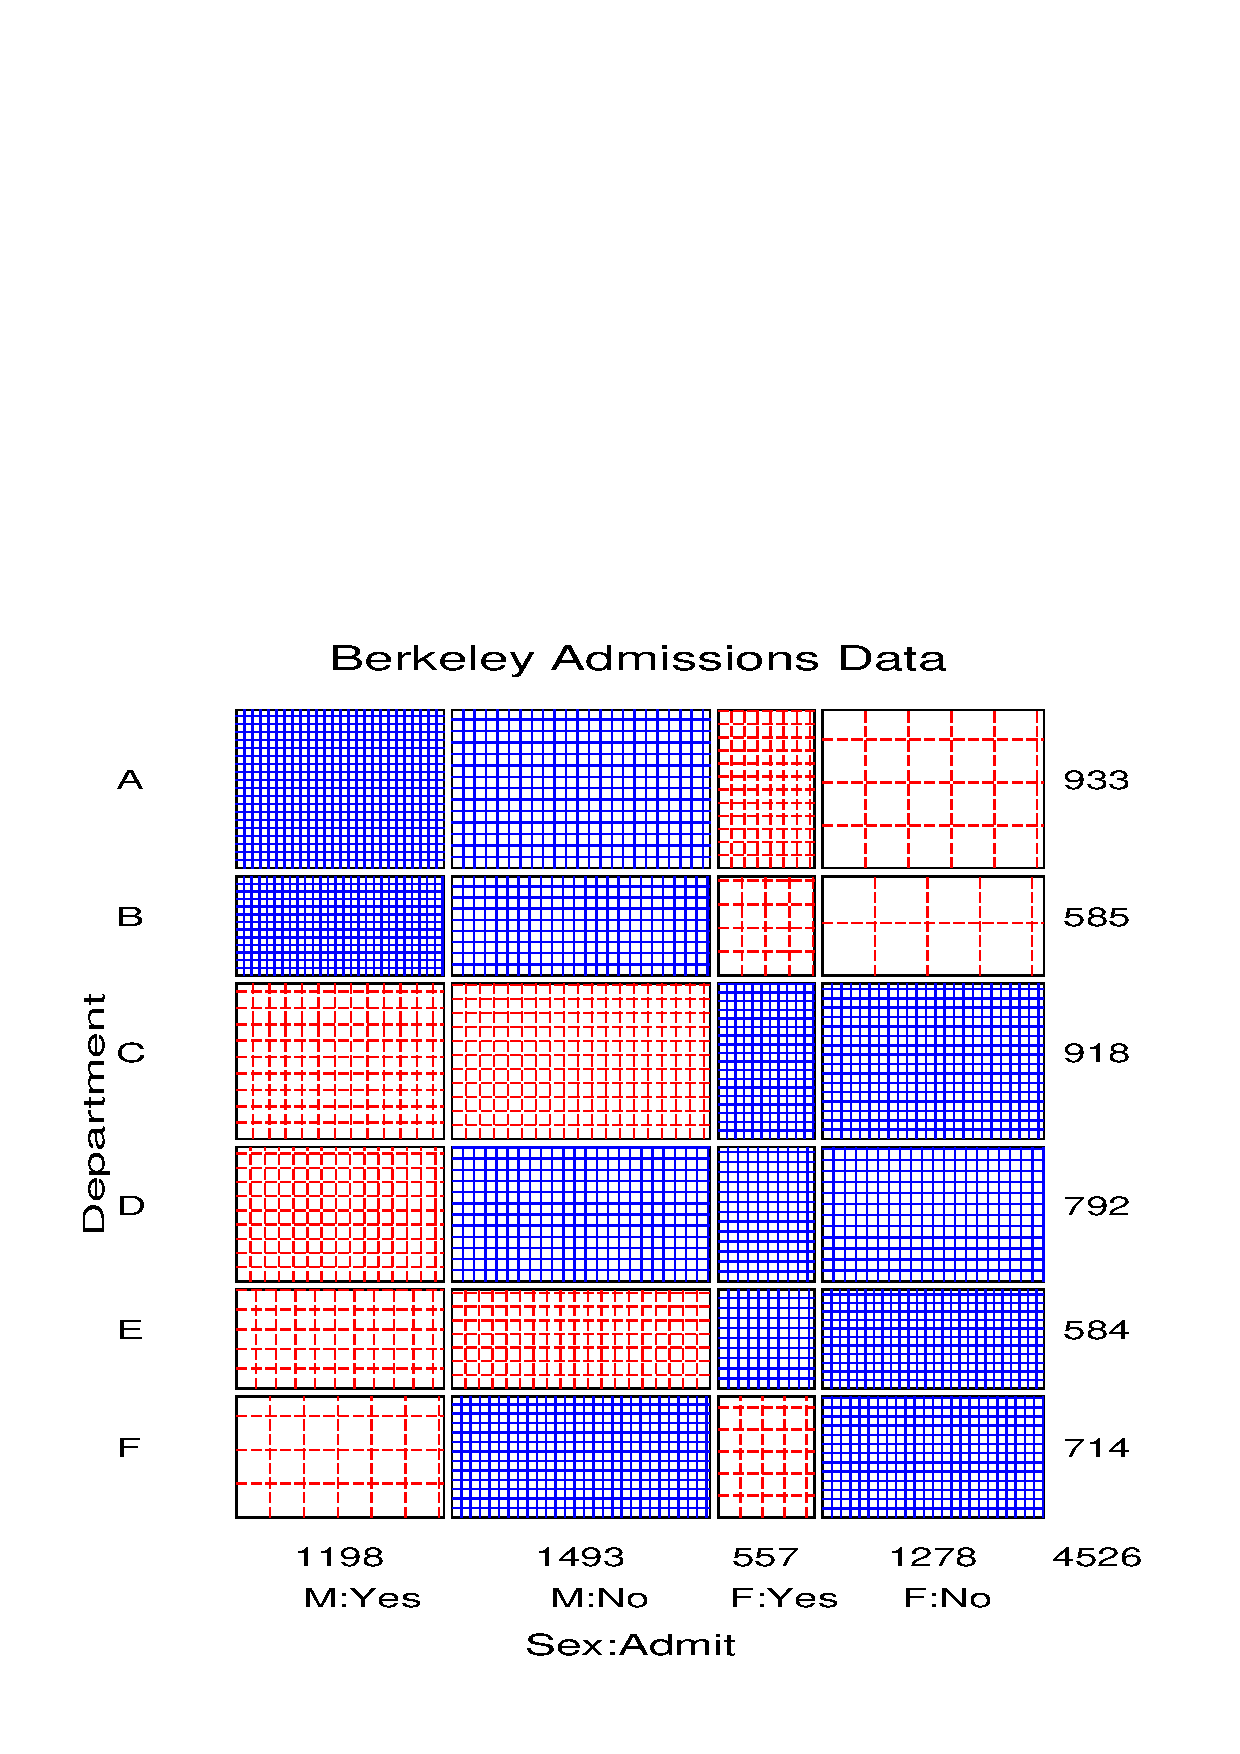
\includegraphics[scale=.6]{ch1/fig/sievebrk1}
  \caption[Sieve diagram for Berkeley admissions data]{Sieve diagram for Berkeley admissions data.  Each box has area proportional to its expected frequency, and is cross-ruled with boxes equal to the observed frequency.}\label{fig:sievebrk1}
\end{figure}
\ix{sieve diagram|)}

The second point is illustrated in \figref{fig:mosdemo},
using data (see \tabref{tab:hairdat}) on $n=592$ individuals
classified by hair color.
In the conceptual model
\citep{Friendly:95,Sall:91b}, categorical observations are likened to
molecules of an ideal gas confined to chambers separated by moveable
partitions.  In both panels of the figure, the number of symbols in each box exactly
equals the number of observations in each hair color category.

%% two subfig side-by-side
\begin{figure}[htb]
 \begin{minipage}[t]{.49\linewidth}
  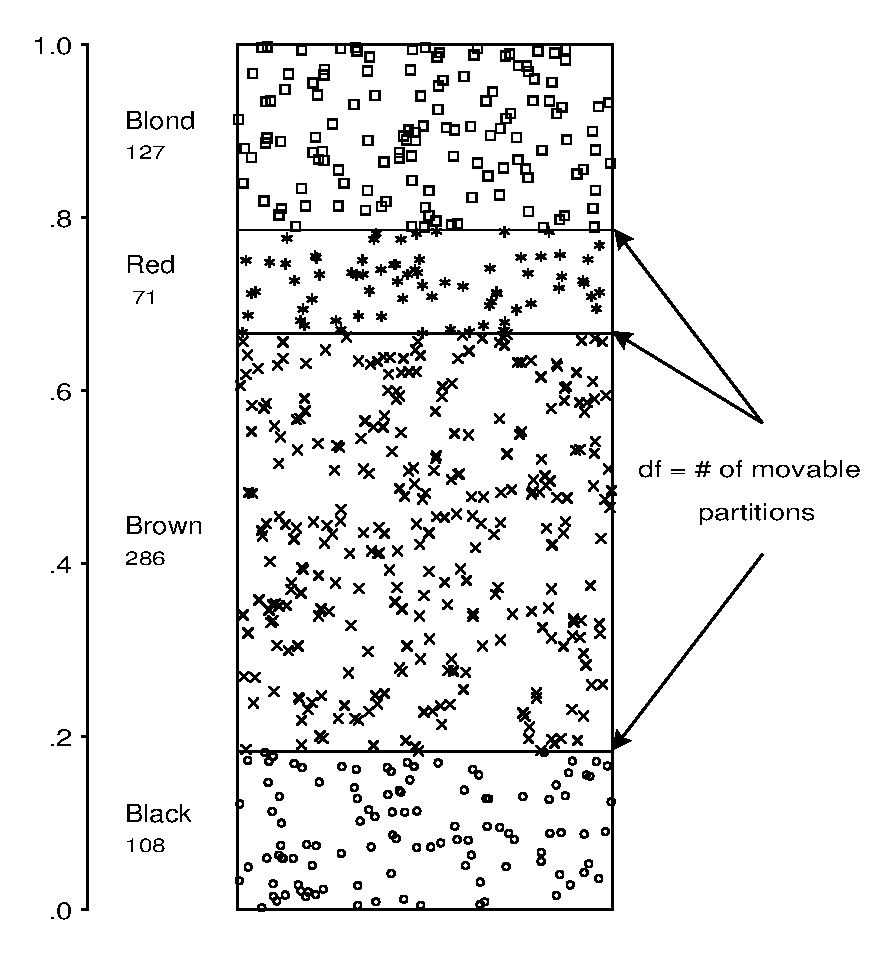
\includegraphics[width=1\linewidth,clip]{ch1/fig/mosdemo3}
 \end{minipage}%
 \hfill
 \begin{minipage}[t]{.49\linewidth}
  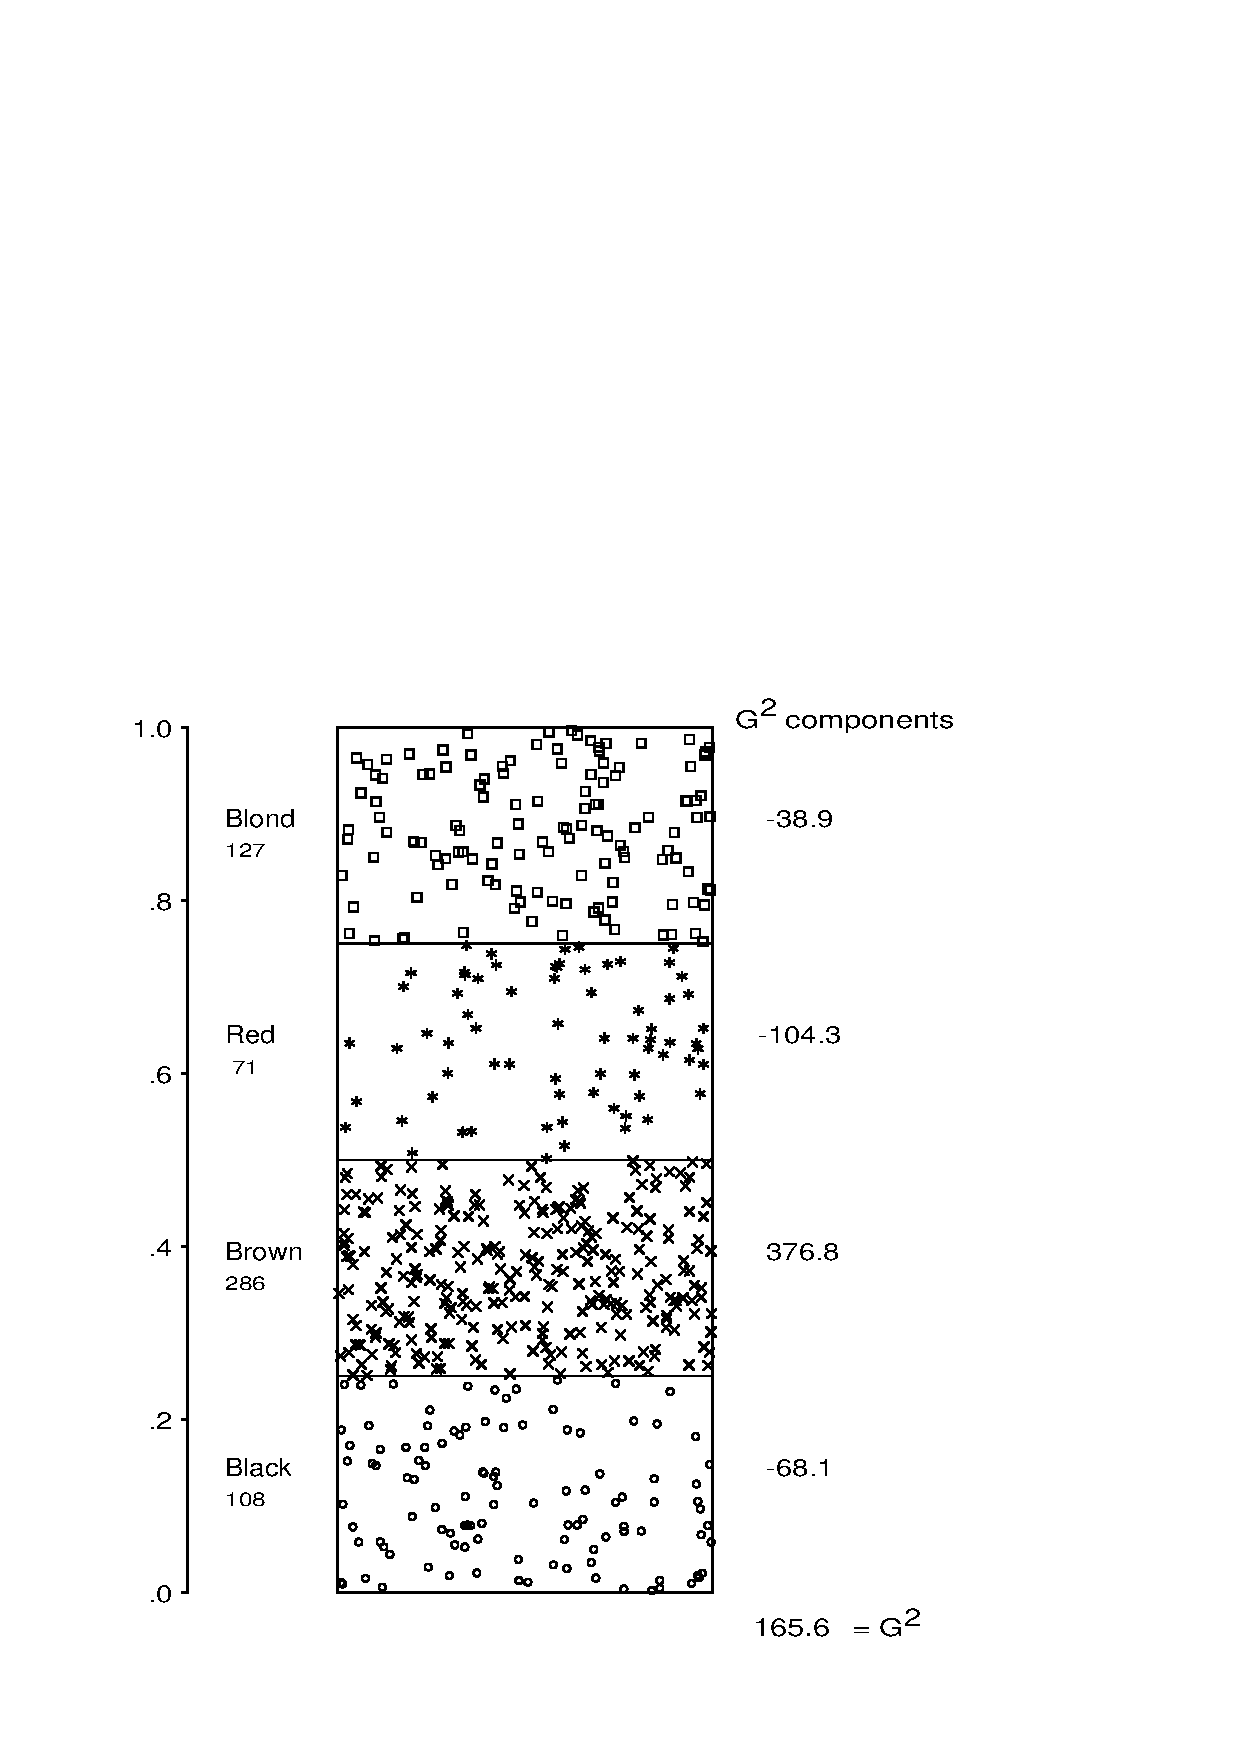
\includegraphics[width=1\linewidth,clip]{ch1/fig/mosdemo4}
 \end{minipage}
 \caption{Conceptual model for categorical data}\label{fig:mosdemo}
\end{figure}

When the location of the partitions are unconstrained, as in the
left panel of \figref{fig:mosdemo}, the forces balance in each chamber
by moving to the positions of minimum potential energy, so that
the height of each chamber is $p_i = n_i / n$, which is the maximum likelihood
estimate of the probability $\pi_i$ in each cell.

To test the hypothesis that all hair colors are equally likely,
imagine forcing the partitions to move to the positions where
$\pi_i = \frac{1}{4}$, as shown in the right panel.
The change in energy in each compartment is then 
$- ( \log  p_i - \log  \pi_i ) = - \log ( p_i / \pi_i )$ , 
the change in negative log-likelihood. Sum these up and multiply by 2 to get the likelihood ratio \GSQ. This gives a concrete interpretation of \GSQ\ as a measure of the effort to maintain belief in the hypothesis in the face of the data. 

This concrete model supplies neat explanations of many other results for categorical data, extends readily to multiway tables, and provides a rationale for the graphic representation of counts by area or visual density.
It also serves as basis for the mosaic display, described in
\chref{ch:mosaic}.

\section{Visualization = Graphing + Fitting + Graphing}\label{sec:intro-visualize}
\epigraph{Look here, upon this picture, and on this.}{Shakespeare, Hamlet}

Statistical summaries, hypothesis tests, and the numerical parameters
derived in fitted models are designed to capture a particular feature of the
data.  An analysis of the data from \tabref{tab:berk220}, for example,
shows that 44.5\% of male applicants were admitted, compared to
30.4\% of female applicants, giving a Pearson chi-square of 92.2
with 1 degree of freedom
for association between admission and gender ($p < 0.001$).
Expressed in terms of the odds ratio, males were apparently
1.84 times as likely
to be admitted as females, with 99\% confidence bounds
1.562--2.170.
Each of these numbers expresses some part of the relationship between
gender and admission in the Berkeley data.

Numerical summaries, even for such a small \Dset\ as this,
are designed to compress the information in the data.
In contrast, the visualization approach to data analysis is designed
to 
\begin{seriate}
\item expose information and structure in the data,
\item supplement the information available from numerical summaries, and 
\item suggest more adequate models.
\end{seriate}
In general, the visualization approach seeks to serve the needs of
both summarization and exposure.

This approach recognizes that both data analysis and graphing are
iterative processes.
We should not expect that any one model captures all features of the
data any more than we should expect that a single graph shows all that
may be seen.  In most cases, our initial steps should include some
graphical display guided by understanding of the subject matter
of the data.
What we learn from a graph may then help suggest features of the data
to be incorporated into a fitted model.
A desire to ensure that the fitted model is an adequate summary
may then lead to additional graphs.

\begin{Example}[lifeboat0]{Lifeboats on the \emph{Titanic}}
One example is shown in \figref{fig:lifeboat}, described in more
detail in \exref{ex:lifeboat1}.
The left panel shows a trilinear plot of the composition of 
lifeboats on the \emph{Titanic}.
Each point in the plot shows the relative proportions of male
passengers
(identifying those with 10\% or more men), women and children and ``men of crew'' reported in each of the
18 lifeboats launched from the port and starboard sides of that
ill-fated vessel.
Trilinear plots are described in \secref{sec:twoway-trilinear},
but essentially, points near the top apex represent boats
nearly all filled with women and children.
%% two subfig side-by-side
\begin{figure}[htb]
 \begin{minipage}[c]{.49\linewidth}
  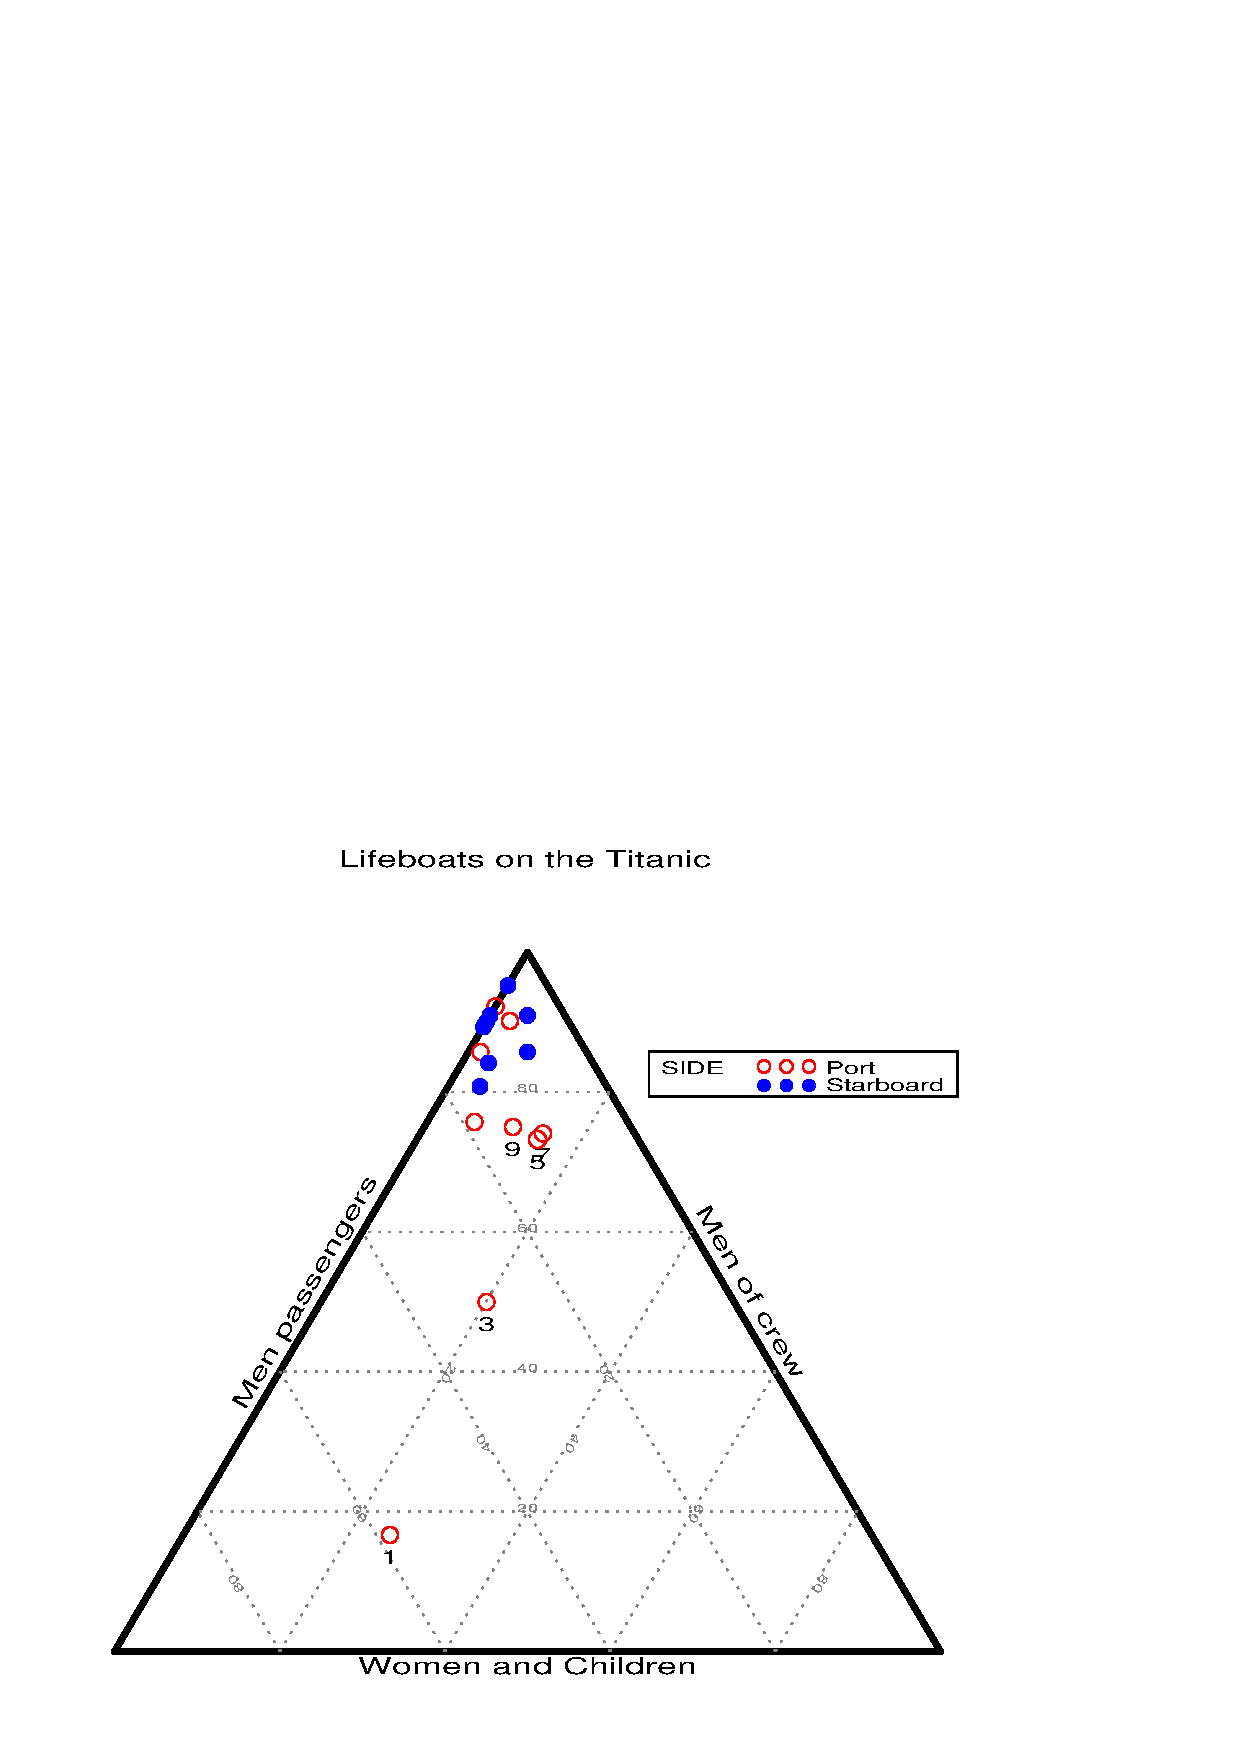
\includegraphics[width=1\linewidth,clip]{ch3/fig/lifeboat1}
 \end{minipage}%
 \hfill
 \begin{minipage}[c]{.49\linewidth}
  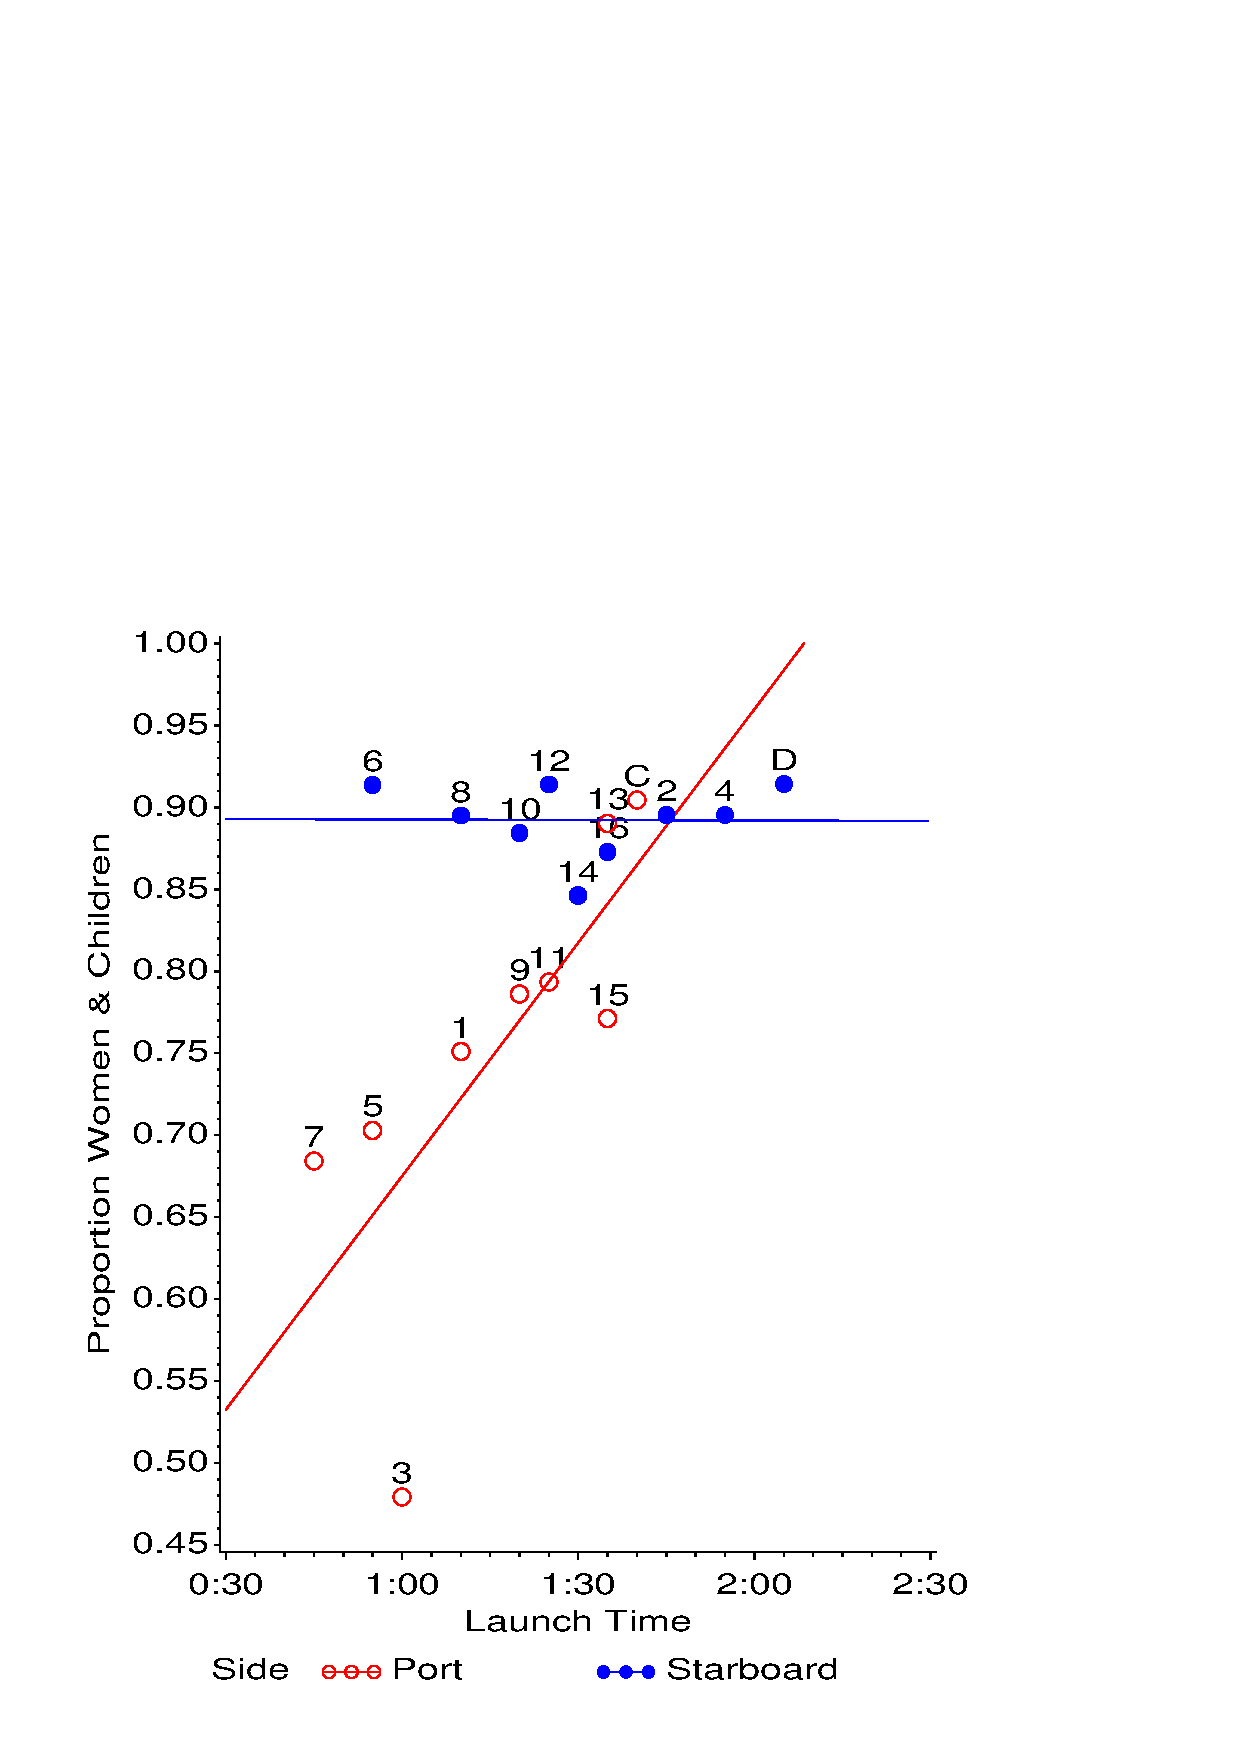
\includegraphics[width=1\linewidth,clip]{ch1/fig/lifeboat3}
 \end{minipage}
 \caption[Two graphical displays for \emph{Titanic} lifeboat data]{Two graphical displays for \emph{Titanic} lifeboat data. Left: trilinear plot, right: logistic regression.}\label{fig:lifeboat}
\end{figure}

That graph suggested that the procedures for loading the lifeboats
might have differed for the port and starboard side of the ship.
We were led to fit a logistic regression model predicting the
proportion of women and children loaded over time, with separate
slopes and intercepts for the port and starboard sides.
The right panel of \figref{fig:lifeboat} shows predicted proportions
from this model, with simple linear regression lines for the
two sides.  Even without further details about the data or
the analysis, the graph shows clearly that passengers on the two
sides of the \emph{Titanic} were subject to different regimes
for loading the lifeboats.
\end{Example}

This interplay between graphing and fitting may be expressed as
\begin{equation*}
\textrm{Visualization} = \textrm{Graphing} + \textrm{Fitting} + \textrm{Graphing} + \cdots
\comma
\end{equation*}
where the $\cdots$ remind us that there are often additional steps.

Sometimes a visualization is sufficiently strong (as, perhaps in
\figref{fig:glogist00} or the right panel of \figref{fig:lifeboat}),
that hypothesis tests and model parameters
serve an ancillary role in understanding the effects in the data. 
$p$-values are useful in the conventions of scientific communication,
but perhaps less convincing evidence than a graph whose conclusions hit you
between the eyes.

In other cases, graphing serves as a supporting member of the data-analytic
cast.  Model-based methods rely on assumptions about the data.
Diagnostic plots for logistic regression (\secref{sec:logist-infl})
and \loglin\ models (\secref{sec:loglin-infl})
may provide comfort that the assumptions on which these inferences
depend are reasonable for the data at hand, or suggest that some modification
of the model would help us rest more easily.

In any event, it is well to remember that data analysis requires both
summarization and exposure, and the needs of both are served by the
combination of graphing and fitting.

\subsection{Static vs.\ dynamic graphics}
\ix{graphics!static vs.\ dynamic|(}
The confines of a book and of the software that we describe here for
visualizing categorical data limit this presentation to static displays,
produced by SAS programs.  Many of these static graphics are made
considerably easier to use and more flexible by a number of SAS macros
illustrated in the following chapters and described in Appendix~\ref{ch:macros}.

The most productive use of these methods will require the addition of
two aspects of interactive graphics, presently being developed
by the author \citep{Friendly:96}
and by others \citep{TheusLauer:99,Young:94}.
\begin{itemize}
\item The first aspect relates to interactive methods for choosing variables,
parameters, and options for analysis and graphical displays.  The 
development tools for this form of interactivity are provided in \AF\
and most of the macro programs described here may be easily wrapped
in an interactive front-end.

\item A second aspect of dynamic graphics is related to the ability to interact
with multiple, linked  views of a \Dset, so that, for example,
selecting a subset of cases in one view highlights them in all other
views.  \INSIGHT\
is a prototype for this type of interaction in the SAS System.

\end{itemize}

We look forward to the development of more interactive methods and the
extension of multiple, linked data views for
categorical data with the SAS System.  Nevertheless, we need to understand
the various forms of graphic displays which are particularly useful
for discrete data before learning how to
employ them interactively.
\ix{graphics!static vs.\ dynamic|)}

